\documentclass[a4paper,12pt]{article}
\usepackage[russian]{babel} % Поддержка русского языка
\usepackage{fontspec}
\setmainfont[Ligatures=TeX]{Times New Roman} % Шрифт для основного текста
\setsansfont[Ligatures=TeX]{Arial}
\setmonofont{Consolas} % Шрифт для кода
\usepackage{amsmath, amssymb} % Для математических формул
\usepackage[left=1.45cm, right=1.45cm, top=1.5cm, bottom=1.5cm]{geometry} % Настройка полей
\usepackage{pdflscape} % Поворот страниц в PDF
\usepackage{graphicx}

\usepackage{xcolor}
\usepackage{enumitem}
\usepackage{ulem}
\usepackage{tcolorbox}

\usepackage{adjustbox}

\usepackage[colorlinks=true]{hyperref}
\hypersetup{
	colorlinks=true,
	linkcolor=blue, % Почему-то зависит от colorlinks=true
}

%-------------------ЦВЕТНОЙ ФОН ФЛОМАСТЕРА-------------------%
% Цвета
\definecolor{lightblue}{RGB}{202,244,255}
\definecolor{pink}{RGB}{255,230,245}

% Цветные боксы
\newtcolorbox{highlightbox}{
	colback=lightblue,
	colframe=lightblue,
	boxrule=0pt,
	arc=3mm,
	auto outer arc,
	boxsep=2mm,
	left=2mm, right=2mm, top=1mm, bottom=1mm
}

\newtcolorbox{pinkbox}{
	colback=pink,
	colframe=pink,
	boxrule=0pt,
	arc=2mm,
	auto outer arc,
	boxsep=1mm,
	left=1mm, right=1mm, top=0.5mm, bottom=0.5mm
}

%-------------------КРУГОВАЯ ОБВОДКА-------------------%
\usepackage{titlesec}
\usepackage{tikz}

% Универсальная команда для обводки
\newcommand{\circled}[1]{%
	\tikz[baseline=(char.base)]{%
		\node[draw,circle,inner sep=1pt,minimum size=1.2em](char){\strut #1};%
	}%
}

% Модифицированная команда для разделов с обведённым номером
\newcommand{\circledsection}[2][]{%
	% \refstepcounter{section} % Раскомментировав - раздел будет считаться в общей нумерации
	\par\vspace{4ex plus 1ex minus .2ex}%
	\noindent{\Large\bfseries\circled{\thesection}~#2\par} % \thesection передает номер из оглавление в раздел
	\addcontentsline{toc}{section}{\protect\numberline{\thesection}#2} % С #1 будет убрано название и останутся только точки
	\vspace{2.5ex plus .2ex}%
}

% Модифицированная команда для подразделов с обведённым номером
\newcommand{\circledsubsection}[1]{%
	\refstepcounter{subsection} % Отвечает за нуммерацию
	\par\vspace{3.25ex plus 1ex minus .2ex}%
	\noindent{\large\bfseries\circled{\thesubsection}~#1\par}%
	\addcontentsline{toc}{subsection}{\protect\numberline{\thesubsection}#1}%
	\vspace{2.3ex plus .2ex}%
}

% Стандартные подразделы
\makeatletter
\renewcommand{\subsection}{\@startsection{subsection}{2}{\z@}%
	{-3.25ex\@plus -1ex \@minus -.2ex}%
	{1.5ex \@plus .2ex}%
	{\normalfont\large\bfseries}%
}
\makeatother

% Реализация списков со сквозной нумерацией (просто \item в них писать не надо)
\newcounter{flexcounter}
\newlist{flexlist}{enumerate}{3}
\setlist[flexlist]{
	before=\setcounter{flexcounter}{0},
	label={\arabic*.},
	ref=\arabic*,
	align=left,
	leftmargin=*,
	labelwidth=!,
	labelindent=0pt
}

\newcommand{\flexlabel}[1]{%
	\ifnum\value{flexcounter}>0\relax%
	\arabic{flexcounter}.%
	\fi%
}

\newcommand{\circleditem}{%
	\refstepcounter{flexcounter}%
	\item[\circled{\arabic{flexcounter}}]%
}

\newcommand{\plainitem}{%
	\refstepcounter{flexcounter}%
	\item[\arabic{flexcounter}]%
}

%-------------------ДЕЛАЕМ ТОЧКИ ОГЛАВЛЕНИЯ АКТИВНЫМИ-------------------%
% Переопределяем \@dottedtocline для полной ссылки
\makeatletter
\def\@dottedtocline#1#2#3#4#5{%
	\ifnum #1>\c@tocdepth \else
	\vskip \z@ \@plus.2pt
	{\leftskip #2\relax
		\rightskip \@tocrmarg \parfillskip -\rightskip
		\parindent #2\relax\@afterindenttrue
		\interlinepenalty\@M
		\leavevmode
		\@tempdima #3\relax
		\begingroup
		\ifnum #1=1 \bfseries \fi % Жирный шрифт только для первого уровня
		\parindent \z@ \leftskip #3\relax
		% \advance\leftskip by 1.5em % - задаем сдвиг подзаголовка
		% \hskip -\leftskip % - двигаем подзаголовок влево
		\hyper@linkstart{link}{\Hy@tocdestname}%
		#4% текст заголовка
		\leaders\hbox{$\m@th
			\mkern \@dotsep mu\hbox{.}\mkern \@dotsep mu$}\hfill
		\nobreak\hb@xt@\@pnumwidth{\hfil #5}% номер страницы
		\hyper@linkend
		\endgroup
		\par}%
	\fi}
% Переопределяем \l@section для использования \@dottedtocline
\renewcommand*\l@section[2]{%
	\ifnum \c@tocdepth >\z@
	\addpenalty\@secpenalty
	\addvspace{1.0em \@plus\p@}%
	\@dottedtocline{1}{0em}{1.5em}{#1}{#2}%
	\fi}
\makeatother

\begin{document}
	
	\tableofcontents
	\newpage
	
	\circledsection{Проверка шаблона}
	\vspace{-2em}
	\circledsubsection{Тестовый пример}
	
	\noindent
	\begin{adjustbox}{valign=m}
		\begin{minipage}[t]{0.65\textwidth}
			\begin{flexlist}
				\circleditem Первый обведённый
				\plainitem Второй обычный
				\circleditem Третий обведённый
				\plainitem Четвертый обычный
				\circleditem Пятый обведённый
			\end{flexlist}
		\end{minipage}
	\end{adjustbox}
	\hspace{1em}
	\begin{adjustbox}{valign=m}
		\begin{pinkbox}
			\makebox[4cm][l]{\circled{A} + \circled{5} = \circled{A5}}
			\par
			Список с русскими буквами:
			{\setcounter{ruscount}{0} % Сбрасываем счетчик
				\rusitem{Первый пункт}
				\rusitem{Второй пункт}
				\rusitem{Третий пункт}
			}
		\end{pinkbox}
	\end{adjustbox}
	
	\section{Понятие модели. Функции моделей. Классификация моделей}

	\subsection{Понятие}
	\textbf{Модель} - это представление объекта системы или понятия в некоторой форме, отличной от формы их реального существования. Это средство, помогающее в объяснении, понимании или совершенствовании системы. Оно способствует пониманию и изменению окружающей среды.
	
	\subsection{Функции моделей}
	\begin{enumerate}
		\item \textbf{Средство осмысления действительности} (реальных связей и закономерностей) 
		\newline
		Правильно построенная модель вынуждает нас организовать свои замыслы, оценить и проверить их обоснованность
		\item \textbf{Средство общения} - она сжато и точно описывает объект, что отличает ее от разговорных языков и делает более понятной общую структуру исследуемого объекта, раскрывая также причинно следственные связи
		\item \textbf{Средство обучения и тренажёра}
		\item \textbf{Инструмент прогнозирования}
		\item \textbf{Средство постановки экспериментов и т.д.}
	\end{enumerate}
	
	\subsection{Классификация моделей}
	\begin{enumerate}
		\item \textbf{Статические и динамические}
		\item \textbf{Детерминированные и стохастические}
		\item \textbf{Дискретные и непрерывные}
		\item \textbf{Физические и натуральные} (+ масштабированные)
		\item \textbf{Аналоговые} (свойства одного объекта через свойства другого)
		\item \textbf{Управленческие игры}
		\item \textbf{Математические модели} (символические)
		\begin{enumerate}
			\item \textbf{Функциональные и структурные} (по характеру отображаемых признаков)
			\item \textbf{По уровню абстракции} - микроуровень, макроуровень, метауровень (\textbf{МММ})
		\end{enumerate}
	\end{enumerate}
	
	\newpage
	
	\section{Модели на микро-, макро- и мета- уровнях. Требования к "хорошей" модели. Основные этапы процесса моделирования}
	
	\subsection{МММ-уровни}
	\textbf{*} Мат. модели с разным уровнем абстракции
	
	\begin{enumerate}
		\item \textbf{Микроуровень:}
		\begin{itemize}
			\item Мат.Модели, описывающие физическое состояние и процессы в сплошных средах
			\item Фазовые переменные - функции многих независимых переменных (непрерывные 
			координаты и время)
			\item Используется для моделирования - аппарат математической физики
			\newline
			(\textbf{\textit{Пр.:}} дифференциальные уравнения в частных производных уравнения электродинамики, теплопроводности, упругости, газовой динамики, отражающие процессы в трехмерной сплошной среде.)
			\item Типовые фазовые переменные: электрические потенциалы, давления, температуры, 
			концентрации частиц, плотность токов, механические напряжения и деформации
			\item Анализ сводится к решению краевых задач математической физики
		\end{itemize}
		\item \textbf{Макроуровень}
		\begin{itemize}
			\item Производится дискретизация пространства и переход от распределенных моделей микроуровня к сосредоточенным моделям
			\item Элементы - системы: резисторы, микропроцессоры, кронштейны, балки, станины, валы и пр.
			\item Типичные фазовые переменные: токи и напряжения, скорости и силы, потоки и давления и т.п.
			\item Характеризуют появление внешних свойств элементов при их взаимодействии между собой и внешней средой
			\item Мат.Модели: обыкновенные дифф. уравнения, превращающиеся в алгебраические и трансцендентные для статических моделей
		\end{itemize}
		\item \textbf{Метауровень}
		\begin{itemize}
			\item Системы - сложные устройства и комплексы
			\item Элементы и внутренние параметры - системы и выходные параметры микроуровня
			\newline 
			(\textbf{\textit{Пр.:}} комп. элементы - процессор, оператива, устройства ввода вывода; выходные параметры - вероятность обслуживания поступивших заявок, среднее время простоя в очереди на обслуживание и т.п.)
			\item Методы: теория автоматического управления, планирование экспериментов, математическая логика, теория массового обслуживания и др.
			\item Приходим к системам дифференциальных, логических уравнений, имитационным моделям систем массового обслуживания
		\end{itemize}
	\end{enumerate}
	\newpage
	\subsection{Принципы построения Мат.Моделей}
	\begin{enumerate}
		\item \textbf{Физический принцип} - полные физические представления об объекте: ограничена классом хорошо изученных объектов
		\item \textbf{Принцип «черного ящика»} - нет информации об элементах и структуре
		\item \textbf{Принцип «серого ящика»}, полуфизический - компромисс между первыми двумя; \newline \textbf{\textit{Пр.:}} задача параметрической идентификации
	\end{enumerate}
	
	\subsection{Требования к «хорошей» модели}
	
	\begin{enumerate}
		\item Простая и понятная
		\item Целенаправленная
		\item Надёжная
		\item Удобная в управлении и общении
		\item Полная
		\item Адаптивная
		\item Допускающая постепенные изменения
	\end{enumerate}

	\begin{pinkbox}
		\textbf{К матмоделям:}
	\end{pinkbox}

	\begin{enumerate}
		\item Адекватная
		\item Универсальная
		\item Экономичная (по затратам вычислительных ресурсов)
	\end{enumerate}
	
	\subsection{Процесс моделирования}
	
	\begin{enumerate}
		\item \uline{Постановка задачи} и определение типа модели (формулируем проблему)
		\item \uline{Формулирование модели}
		\item \uline{Проверка модели на <<правдивость>>} (правдивость результатов) + установка исходных предположений и серия проверок:
		\begin{itemize}
			\item параметрам задают предельные значения
			\item проверяют исходные предположения
			\item проверяют преобразование информации от входа к выходу
		\end{itemize}
	\end{enumerate}
	
	\newpage
	
	\section{Анализ линейных математических моделей, основные его этапы. Фазовые портреты для моделей первого и второго порядка}
	
	\subsection{Фазовые портреты}
	
	Для геометрической иллюстрации решений (как линейных, так и нелинейных):
	\begin{equation}
		\mathbf{\frac{dx}{dt} = f(x), \quad x(0) = x_0}
	\end{equation}
	
	Строят \textbf{фазовый портрет} — множество траекторий, описыв. поведение реш. в фазовом пространстве.
	\par
	\textbf{Фазовое пространство} — это пространство, где оси соответствуют переменным системы.
	\par
	\vspace{0.5em}
	$\bullet$ Для уравнений 1-го порядка типы траекторий:
	{\setcounter{ruscount}{0} % Сбрасываем счетчик
		\rusitem{Одноточечная (равновесие).}
		\rusitem{Интервал (концы - равновесия).}
		\rusitem{Полупрямая (один конец - равновесие, другой - $\pm\infty$).}
	}
	
	При $f(x) > 0$ движение слева направо, при $f(x) < 0$ — справа налево. 
	\par
	\vspace{0.5em}
	Примеры траекторий:
	\begin{figure}[H]
		\begin{minipage}[t]{0.4\textwidth}
			\begin{itemize}
				\item $x' = x^2$;
				\item $x' = x^3$;
				\item $x' = \frac{1}{2}(x^2 - 1)$;
				\item $x' = \sin(\pi x)$.
			\end{itemize}
		\end{minipage}
		\hspace{-3cm} % Регулировка горизонтального расстояния
		\begin{minipage}[t]{0.45\textwidth}
			\vspace{-0.5\baselineskip} % Корректировка вертикального положения
			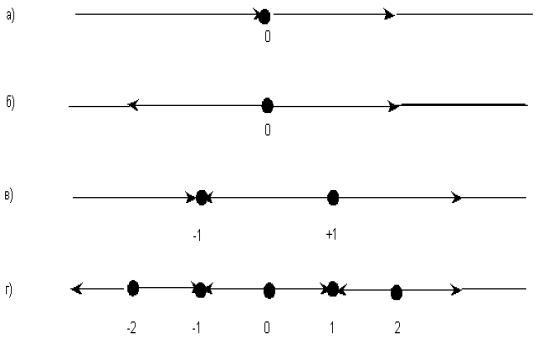
\includegraphics[
			width=\linewidth,
			height=3.3cm,
			keepaspectratio=false
			]{img/3_01}
			\vspace{-3mm} % Поднимает подпись
			\hspace*{4em} % Сдвигает подпись вправо
			{\small \centering Примеры фазовых траекторий}
		\end{minipage}
	\end{figure}
	
	$\bullet$ Для уравнений 2-го порядка существуют линейные системы, матрица 2x2, разные $\lambda_k$.
	
	\vspace{-0.5em}
	\subsection{Линейные системы и их фазовые портреты}
	
	Система:
	\begin{equation}
		\frac{d x}{d t} = A x
	\end{equation}
	
	Точка $x = 0$ — очевидная точка равновесия. 
	\newline
	Пусть $\lambda_k$, $u_k$ - собственные значения и векторы матрицы $A$, а $U$ - матрица с векторами $u_k$ в столбцах.
	\vspace{-1.5em}
	\begin{align}
		A u_k &= \lambda_k u_k, \quad U = (u_1, u_2), \notag \\
		A U &= U \Lambda, \quad \Lambda = U^{-1} A U = \operatorname{diag}(\lambda_1, \lambda_2)
	\end{align}
	
	Замена $x = U y$ приводит систему к диагональному виду:
	
	\begin{equation}
		\frac{d \mathbf{y}}{d t} = \Lambda \mathbf{y}, \quad \Lambda = \begin{pmatrix} \lambda_1 & 0 \\ 0 & \lambda_2 \end{pmatrix}
	\end{equation}
	
	Уравнения:
	\begin{equation}
		\frac{d y_1}{d t} = \lambda_1 y_1, \quad \frac{d y_2}{d t} = \lambda_2 y_2
	\end{equation}
	
	Решения:
	\begin{equation}
		y_1(t) = C_1 e^{\lambda_1 t}, \quad y_2(t) = C_2 e^{\lambda_2 t}
	\end{equation}
	
	\newpage
	Рассмотрим различные сочетания собственных значений:
	
	\begin{pinkbox}
		\subsection*{Вариант 1. Одного знака}
	\end{pinkbox}
	
	\begin{enumerate}
		\item $\lambda_1 < 0$, $\lambda_2 < 0$ (например, $\lambda_1 = -1$, $\lambda_2 = -2$):
		\begin{equation}
			y_1(t) = C_1 e^{-t}, \quad y_2(t) = C_2 e^{-2t}
		\end{equation}
		\vspace{-0.4em}
		$y_2(t) = C_3 y_1^2(t)$, $C_3 = \frac{C_2}{C_1^2}$ — \textbf{устойчивый узел} (парабола).
		\item $\lambda_1 > 0$, $\lambda_2 > 0$ (например, $\lambda_1 = 1$, $\lambda_2 = 2$):
		\begin{equation}
			y_1(t) = C_1 e^{t}, \quad y_2(t) = C_2 e^{2t}
		\end{equation}
		\vspace{-0.4em}
		$y_2(t) = C_3 y_1^2(t)$, $C_3 = \frac{C_2}{C_1^2}$ — \textbf{неустойчивый узел}.
	\end{enumerate}
	В обоих случаях при $C_1 = 0$ и $C_2 = 0$ получаем траектории на оси абсцисс или ординат
	\vspace{-0.5em}
	\begin{figure}[H]
		\centering
		\begin{minipage}[b]{0.49\linewidth}
			\centering
			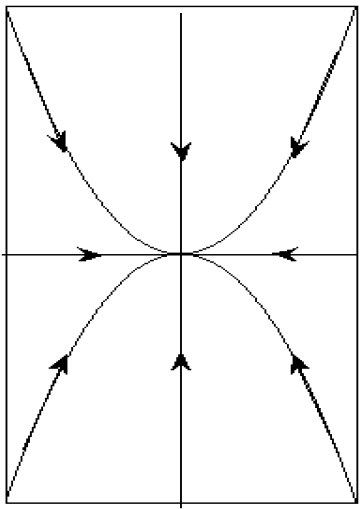
\includegraphics[width=0.5\linewidth]{img/3_02}
			\par
			\small Устойчивый узел
		\end{minipage}
		\hfill
		\begin{minipage}[b]{0.49\linewidth}
			\centering
			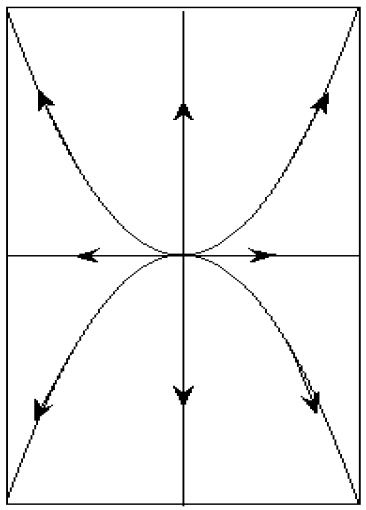
\includegraphics[width=0.5\linewidth]{img/3_03}
			\par
			\small Неустойчивый узел
		\end{minipage}
	\end{figure}
	
	\begin{pinkbox}
		\subsection*{Вариант 2. Разного знака}
	\end{pinkbox}
	
	$\lambda_1 > 0$, $\lambda_2 < 0$ (например, $\lambda_1 = 1$, $\lambda_2 = -1$):
	\newline
	\begin{equation}
		y_1(t) = C_1 e^{t}, \quad y_2(t) = C_2 e^{-t}
	\end{equation}
	$y_2(t) = \frac{C_3}{y_1(t)}$, $C_3 = C_1 \cdot C_2$ — гипербола (седло).
	\par
	\vspace{0.5em}
	при $C_1 = 0$ и $C_2 = 0$ получаем траектории на оси абсцисс или ординат
	
	\begin{figure}[H]
		\centering
		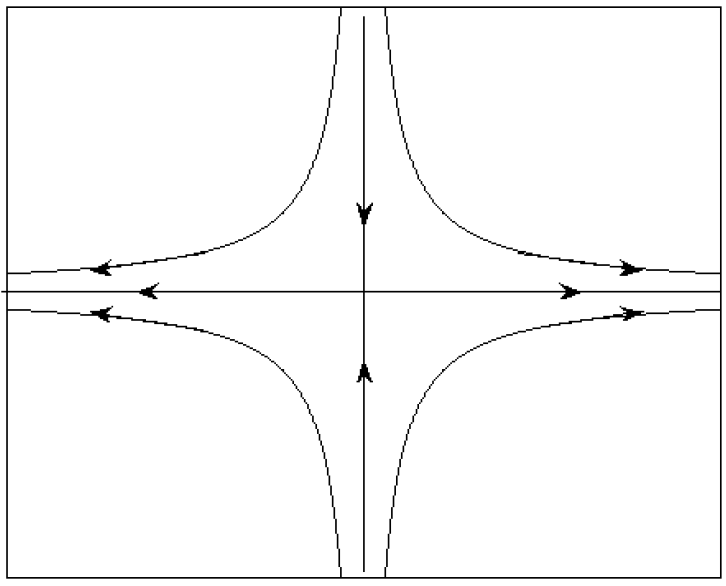
\includegraphics[width=0.4\textwidth, height=0.2\textheight]{img/3_04}
		\par
		\small Равновесие типа «седло»
	\end{figure}
	
	\begin{pinkbox}
		\subsection*{Вариант 3. Комплексно-сопряжённые}
	\end{pinkbox}
	
	$\lambda_{1,2} = \alpha \pm i \omega$:
	\begin{equation}
		y_1(t) = C_1 e^{\alpha t} \cos(\omega t), \quad y_2(t) = C_2 e^{\alpha t} \sin(\omega t)
	\end{equation}
	При $C_1 = C_2 = 1$:
	\begin{equation}
		y_1^2 + y_2^2 = e^{2 \alpha t}
	\end{equation}
	$\alpha < 0$ — устойчивый фокус, $\alpha > 0$ — неустойчивый фокус.
	
	\begin{figure}[H]
		\centering
		\begin{minipage}[b]{0.49\linewidth}
			\centering
			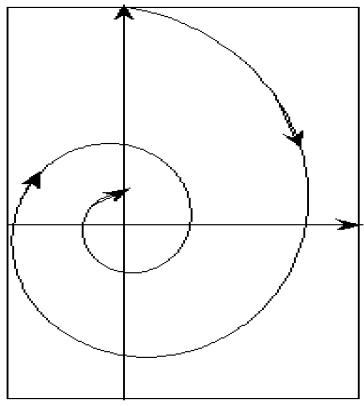
\includegraphics[width=0.7\linewidth]{img/3_05}
			\par
			\small Устойчивый фокус
		\end{minipage}
		\hfill
		\begin{minipage}[b]{0.49\linewidth}
			\centering
			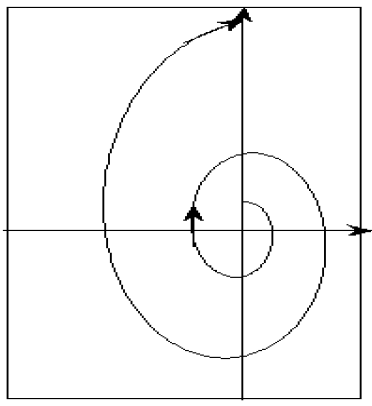
\includegraphics[width=0.7\linewidth]{img/3_06}
			\par
			\small Неустойчивый фокус
		\end{minipage}
	\end{figure}
	
	\subsection{Нелинейные системы}
	В малой окрестности точки равновесия нелинейную систему можно сколь угодно точно аппроксимировать линейной, поэтому поведение её решений соответствует типовым фазовым портретам.
	
	\subsection{Анализ линейных моделей и его этапы}
	
	Линейная динамическая модель с постоянной матрицей:
	\[
		\frac{d \mathbf{x}}{dt} = \mathbf{A} \mathbf{x} + \mathbf{b}
	\]
	где \(\mathbf{x} \in \mathbb{R}^m\) — вектор состояния, \(\mathbf{A}\) — постоянная матрица, \(\mathbf{b}\) — вектор свободных членов.
	\par
	\textbf{Этапы:}
	\begin{enumerate}[label=\arabic*.]
		\item Получение решения
		\item[1a.] Получение стационарного решения и анализ его устойчивости
		\item Определение наблюдаемости отдельных составляющих решения, оценка их роли в системе
		\item Оценка чувствительности к параметрам (и к нежелательным эффектам, и к параметрам для решения)
		\item Решение задачи параметрической идентификации
		\item Решение задачи управления или выбора оптимальных значений параметров
	\end{enumerate}
	
	\newpage
	
	\section{Получение решения линейной модели (построение матричной экспоненты и интеграла от нее)}
	
	Линейные динамические модели описываются дифференциальным уравнением вида
	\begin{equation}
		\frac{d \mathbf{x}}{d t} = \mathbf{A} \mathbf{x} + \mathbf{b},
	\end{equation}
	где \(\mathbf{x} \in \mathbb{R}^m\) — вектор состояния, \(\mathbf{A}\) — постоянная матрица, \(\mathbf{b}\) — вектор свободных членов.
	\par
	\subsection{Основные этапы анализа (1 - 1a - 2)}
	\begin{enumerate}
		\item Получение решения
		\item[1a.] Получение стационарного решения и анализ его устойчивости
		\item Определение наблюдаемости и модальный анализ
		\item Оценка чувствительности к параметрам
		\item Параметрическая идентификация
		\item Задачи управления
	\end{enumerate}
	
	\subsubsection{Этап 1a: Получение стацион. решения и анализ устойчивости}
	Требует решения СЛАУ:
	\begin{equation}
		A x + b = 0, \quad x^* = -A^{-1} b.
	\end{equation}
	\begin{itemize}
		\item Используются программы \textbf{DECOMP} и \textbf{SOLVE} для вычисления.
		\item Устойчивость проверяется \textbf{QR}-алгоритмом, вычисляющим \(\lambda_k\) матрицы \(A\).
		\item Условие асимптотической устойчивости: \(\operatorname{Re} \lambda_k < 0\).
	\end{itemize}
	\subsubsection{Этап 1: Получение решения $\frac{d \mathbf{x}}{d t} = \mathbf{A} \mathbf{x} + \mathbf{b}$}
	Систему~ можно решать стандартными методами (например, \textbf{RKF45}), но использование её линейных свойств повышает надёжность и эффективность, особенно при жёсткости.
	\begin{itemize}[leftmargin=1em]
		\item \textbf{Точное решение} имеет вид:
		\begin{equation}
			x(t) = e^{A t} x_0 + \int_0^t e^{A \tau} d \tau \cdot b.
			\label{eq:14}
		\end{equation}
		\begin{itemize}
			\item Проблема: для больших \(t\) сходимость рядов медленная
			\item Метод \textbf{Ракитского} - предварительные матричные преобразования: 
			\par
			Пусть \( t_n = nH \). Запишем решение уравнения~\eqref{eq:14} в точке \( t_{n+1} = t_n + H \)
			
			\begin{equation}
				x(t_n + H) = e^{A H} x(t_n) + \int_0^H e^{A \tau} d \tau \cdot b.
			\end{equation}
			\item Доказательство:
			\par
			Вычтем из него формулу~\eqref{eq:14}, предварительно умноженную на \( e^{AH} \)
			\begin{align}
				\hspace{-1.5em}x(t_n + H) - e^{A H} x(t_n) &= \int_0^{t_n + H} e^{A \tau} d \tau \cdot b - e^{A H} \int_0^{t_n} e^{A \tau} d \tau \cdot b = \int_0^H e^{A \tau} d \tau \cdot b.
				\label{eq:15}
			\end{align}
		\end{itemize}
		\item \textbf{Аппроксимация рядов}
		\par
		В отличие от~\eqref{eq:14}, формула~\eqref{eq:15} требует \uline{однократного} вычисления \( e^{AH} \) и интеграла, после чего \( x(t_n) \) находится пошагово с шагом \( H \). Для вычислений используем степенные разложения:
		\begin{equation}
			e^{A H} \cong E + H A + \frac{H^2 A^2}{2} + \cdots,
		\end{equation}
		\begin{equation}
			\int_0^H e^{A \tau} d \tau \cong H \left( E + \frac{H A}{2} + \frac{H^2 A^2}{6} + \cdots \right).
		\end{equation}
		При больших по модулю показателях экспоненты ряд сходится медленно. Если матрица \(A\) диагонализуема, \(e^{AH}\) представляется в виде:
		\begin{equation}
			e^{AH} = U
			\begin{pmatrix}
				e^{\lambda_1 H} & \cdots & 0 \\
				\vdots & \ddots & \vdots \\
				0 & \cdots & e^{\lambda_m H}
			\end{pmatrix}
			U^{-1}.
		\end{equation}
		\begin{itemize}
			\item Для жестких систем: \(h = \frac{H}{2^N}\), \(\|A\| h < 1\).
			\item Вычисление: \(e^{A H} = (e^{A h})^{2^N}\) с \(e^{2 A h} = e^{A h} \cdot e^{A h}\).
			\par
			\item Вектор: \(g(h) = \int_0^h e^{A \tau} d \tau \cdot b\), \(g(2h) = (E + e^{A h}) g(h)\).
			\par
			Пояснение:
			\begin{equation}
				\begin{aligned}
				g(2h) & = \int_0^{2h} e^{A\tau} d\tau \cdot b = \int_0^h e^{A\tau} d\tau \cdot b + \int_h^{2h} e^{A\tau} d\tau \cdot b = \nonumber\\
				& \hspace{-2em}= \int_0^h e^{A\tau} d\tau \cdot b + e^{Ah} \int_0^h e^{A\tau} d\tau \cdot b = (E + e^{Ah}) g(h).
				\end{aligned}
			\end{equation}
		\end{itemize}
		\item \textbf{Резюме алгоритма решения}
		\begin{enumerate}
			\item Задавая конечный шаг наблюдения $H$, выбираем целое $N$: 
			\(h = \frac{H}{2^N} < \frac{1}{|\Lambda|}\)
			\item Для шага $h$ строим матричную экспоненту $e^{Ah}$ и вектор $g(h)$ разложением в ряд с небольшим числом членов
			\item Получаем матрицу $e^{AH}$ и вектор $g(H)$, используя $N$ раз формулу удвоения шага
			\item Решаем уравнение пошаговым методом
		\end{enumerate}

		На основе изложенного алгоритма написана программа \textbf{LSODE}:
		\newline
		Вызов:
		\(\textbf{LSODE}(N, H, CH, A, B, X, EAH, SL, INDEX)\)
		
		\begin{itemize}[leftmargin=1.5em]
			\item $N$ — размерность системы
			\item $H$ — шаг наблюдения решения
			\item $CH$ — константа для оценки начального шага $h$ (для обычных 0.1, для жёстких 5.0)
			\item $A$, $B$ — матрица и вектор системы
			\item $X$ — вектор решения
			\item $EAH$ — матрица, содержащая элементы матрицы $e^{AH}$
			\item $SL$ — рабочий массив размерности $N$
			\item $INDEX$ — управляющий параметр со входными значениями:
			\begin{itemize}
				\item \textbf{1} — первое обращение, вектор $B$ нулевой (т.е. однородная система)
				\item \textbf{2} — первое обращение, $B$ может быть ненулевым
				\item \textbf{0} — последующее обращение
				\item Нормальное выходное значение – \textbf{0}. 
			\end{itemize}
		\end{itemize}
	\end{itemize}
	
	\newpage
	
	\subsubsection{Этап 2: Наблюдаемость и модальный анализ}
	Пусть $\lambda_k$, $u_k$ — собственные значения и собственные векторы матрицы $A$, 
	\newline
	а $\lambda_k$, $v_k$ — собственные значения и собственные векторы матрицы $A^\top$ соответственно.
	\vspace{-1em}
	\subsubsection*{Собственные векторы и их свойства}
	
	\begin{itemize}[leftmargin=1em]
		\item \textbf{Уравнения для собственных векторов:}
		\begin{align}
		A u_k &= \lambda_k u_k, \label{eq:21}\\
		\quad A^T v_i &= \lambda_i v_i \quad \text{или} \quad v_i^T A = \lambda_i v_i^T. \label{eq:22}
		\end{align}
		\item \textbf{Ортогональность:}
		\begin{itemize}
			\item Умножим \eqref{eq:21} слева на \(v_i^T\), \eqref{eq:22} справа на \(u_k\), и вычтем результаты:
			\begin{equation}
				v_i^T A u_k - \lambda_k v_i^T u_k = \lambda_i v_i^T u_k - \lambda_k v_i^T u_k,
			\end{equation}
			\begin{equation}
				(\lambda_i - \lambda_k) v_i^T u_k = 0.
			\end{equation}
			\item Если \(k \neq i\), то
			\begin{equation}
				v_i^T u_k = 0. \label{eq:25}
			\end{equation}
		\end{itemize}
		\item \textbf{Нормировка:}
		\begin{equation}
			v_k^T u_k = 1.
		\end{equation}
	\end{itemize}
	
	\subsubsection*{Формула Лагранжа-Сильвестра}
	
	\begin{itemize}
		\item \textbf{Начальная форма:}
		\begin{equation}
			\hspace{-3em}f(A) = \sum_{k=1}^m T_k f(\lambda_k), \quad T_k = \frac{(A - \lambda_1 E) \cdots (A - \lambda_{k-1} E)(A - \lambda_{k+1} E) \cdots (A - \lambda_m E)}{(\lambda_k - \lambda_1) \cdots (\lambda_k - \lambda_{k-1})(\lambda_k - \lambda_{k+1}) \cdots (\lambda_k - \lambda_m)}.
		\end{equation}
		\item \textbf{Свойства \(T_k\):}
		\begin{itemize}
			\item Если \(k \neq i\), то \((A - \lambda_i E) u_i = 0\), следовательно,
			\begin{equation}
				T_k u_i = 0. \label{eq:28}
			\end{equation}
			\item Для \(k = i\),
			\begin{equation}
				T_k u_k = u_k.
			\end{equation}
		\end{itemize}
		\item \textbf{Разложение \(T_k\):}
		\begin{itemize}
			\item Представим \(T_k = \sum_{j=1}^m c_j v_j^T\) (разложив каждую строку по векторам \(v_j^T\)).
			\item Из~\eqref{eq:25} и~\eqref{eq:28}:
			\begin{equation}
				T_k u_i = \sum_{j=1}^m (c_j v_j^T)u_i = \sum_{j=1}^m c_j (v_j^T u_i) = c_i (v_i^T u_i) = 0, \quad k \neq i,
			\end{equation}
			\begin{equation}
				T_k u_k = c_k (v_k^T u_k) = c_k = u_k.
			\end{equation}
			\item Следовательно,
			\begin{equation}
				T_k = u_k v_k^T.
			\end{equation}
		\end{itemize}
		\item \textbf{Итоговая форма:}
		\begin{equation}
			f(A) = \sum_{k=1}^m u_k v_k^T f(\lambda_k).
		\end{equation}
	\end{itemize}
	
	\newpage
	
	\section{Наблюдаемость отдельных составляющих решения линейной системы. Пример программы модального анализа}
	
	\subsection{Основные этапы анализа (2 - продолжение)}
	
	\subsubsection{Этап 2: Наблюдаемость отдельных составляющих решения}
	
	\subsubsection*{Мода. Решение однородной системы}
	
	\begin{itemize}
		\item \textbf{Общее решение:}
		\begin{equation}
			x(t) = e^{A t} x_0 = \sum_{k=1}^{m} u_k v_k^{T} e^{\lambda_k t} x_0 
			= \sum_{k=1}^{m} u_k \left( v_k^{T} x_0 \right) e^{\lambda_k t}
		\end{equation}
		где \(e^{\lambda_k t}\) — \textbf{мода}, а анализ характера ее поведения в решении – \textbf{модальный анализ}.
		\item \textbf{Покомпонентное решение:}
		\begin{itemize}
			\item Для \(b = 0\) из уравнения $\frac{d \mathbf{x}}{d t} = \mathbf{A} \mathbf{x} + \mathbf{b}$:
			\begin{equation}
				x(t) = \sum_{k=1}^m u_k v_k^T e^{\lambda_k t} x_0.
			\end{equation}
			\begin{equation}
				x^{(p)}(t) = \sum_{k=1}^m u_k^{(p)} D_k e^{\lambda_k t}, \quad D_k = v_k^T x_0.
			\end{equation}
			\item Компоненты:
			\begin{equation}
				x^{(1)}(t) = u_1^{(1)} D_1 e^{\lambda_1 t} + \cdots + u_m^{(1)} D_m e^{\lambda_m t},
			\end{equation}
			\begin{equation}
				x^{(m)}(t) = u_1^{(m)} D_1 e^{\lambda_1 t} + \cdots + u_m^{(m)} D_m e^{\lambda_m t}.
			\end{equation}
		\end{itemize}
		\item \textbf{Отношение амплитуд:}
		\begin{equation}
			\eta_k^{(p,s)} = \frac{x^{(p)}(t)}{x^{(s)}(t)} = \frac{u_k^{(p)} D_k}{u_k^{(s)} D_k} = \frac{u_k^{(p)}}{u_k^{(s)}},
		\end{equation}
		не зависит от \(x_0\).
	\end{itemize}
	
	\subsubsection*{Упрощения}
	\begin{enumerate}
		\item Пусть система из \(m\) однотипных узлов
		\item Поведение узлов описывается $\dfrac{dx^{(p)}}{dt} = \dots$
		\item Все $x^{(p)}(t)$ имеют одинаковую физическую природу и размерность
		\item Структура $A$ определяет функционирование системы целиком
		\item Преимущества будем задавать вектором начальных условий $x_0 = e_i = (0, 0, \dots, 0, 1, 0, \dots 0, 0)^T$, где одна компонента = 1
	\end{enumerate}
	
	\newpage
	
	\subsubsection*{Пример программы модального анализа}
	\begin{itemize}
		\item \textbf{Подсистема 1: Оценка поведения $k$-й моды $e^{\lambda_k t}$}
		\begin{itemize}
			\item Входной параметр: номер моды $k$.
			\item Анализирует наблюдаемость моды в узлах системы.
			\item Результат: таблица относительных амплитуд $\left|\eta_k^{(p,s)}\right|\cdot 100\%$, упорядоченных по убыванию.
			\item Определяет системные (заметные в многих узлах) и локальные моды.
			\item Отвечает на вопрос: где возмущение дает максимальную амплитуду моды (по компонентам $\mathbf{v}_k$).
		\end{itemize}
		\begin{table}[H]
			\centering
			\begin{minipage}{0.48\textwidth}
				\centering
				{\small Наблюдаемость $k$-й моды}
				\begin{tabular}{c | c}
					\toprule
					Номер узла & Относительная амплитуда \\
					\midrule
					14 & 100\% \\
					3 & 92\% \\
					115 & 14\% \\
					7 & 0,2\% \\
					\bottomrule
				\end{tabular}
			\end{minipage}
			\hfill
			\begin{minipage}{0.48\textwidth}
				\centering
				{\small Возмущаемость $k$-й моды}
				\begin{tabular}{c | c}
					\toprule
					Номер узла & Относительная амплитуда \\
					\midrule
					14 & 100\% \\
					6 & 78\% \\
					217 & 9\% \\
					29 & 0,05\% \\
					\bottomrule
				\end{tabular}
			\end{minipage}
		\end{table}
		
		\item \textbf{Подсистема 2: Наблюдение в $k$-м узле}
		\begin{itemize}
			\item Входной параметр: номер узла $k$.
			\item Анализирует составляющую $x^{(k)}(t) = \sum_{j=1}^m u_j^{(k)} D_j e^{\lambda_j t}$.
			\item Задача: определить моду с максимальной амплитудой $u_j^{(k)} D_j$ и упорядочить моды по убыванию амплитуд.
			\item Для каждой моды указывается узел, где возмущение максимально эффективно.
		\end{itemize}
		\begin{table}[H]
			\centering
			{\small Наблюдение в $k$-м узле}
			\par
			\begin{tabular}{c | c | c}
				\toprule
				Номер моды & Относительная амплитуда & Эффективный узел возмущения \\
				\midrule
				4 & 65\% & 7 \\
				13 & 15\% & 14 \\
				6 & 14\% & 113 \\
				25 & 3\% & 3 \\
				\bottomrule
			\end{tabular}
		\end{table}
		
		\item \textbf{Подсистема 3: Возмущение в $k$-м узле}
		\begin{itemize}
			\item Входной параметр: номер узла $k$.
			\item Анализирует последствия возмущения $\mathbf{x}_0 = \mathbf{e}_k$.
			\item Задача: определить, какая мода и с какой амплитудой максимально проявляется в узлах системы.
			\item Указывает наиболее эффективный узел наблюдения.
		\end{itemize}
		\begin{table}[H]
			\centering
			{\small Возмущение в $k$-м узле}
			\par
			\begin{tabular}{c | c | c}
				\toprule
				Номер моды & Относительная амплитуда & Эффективный узел наблюдения \\
				\midrule
				8 & 58\% & 2 \\
				23 & 20\% & 16 \\
				2 & 16\% & 102 \\
				35 & 3\% & 4 \\
				\bottomrule
			\end{tabular}
		\end{table}
	\end{itemize}
	
	\newpage
	
	\section{Анализ чувствительности. Чувствительность составляющих решений к вариации параметров}
	\subsection{Основные этапы анализа (3)}
	\subsubsection{Этап 3: Оценка чувствительности к параметрам}
	\begin{itemize}[leftmargin=1em]
		\item \textbf{Статическая модель:} \(f(x(k)) = 0\),
		\begin{equation}
			a_{ij} = \frac{\partial x^{(i)}}{\partial k^{(j)}}
		\end{equation}
		Пусть $A_j$ - $j$-й столбец матрицы, $e_j$ - 
		$j$-й столбец ед. матрицы, а $\Delta k$ - приращение по параметру:
		\begin{equation}
			 A_j \approx \frac{x(k + \Delta k \cdot e_j) - x(k)}{\Delta k},
		\end{equation}
		или более точно:
		\begin{equation}
			A_j \approx \frac{x(k + \Delta k \cdot e_j) - x(k - \Delta k \cdot e_j)}{2 \Delta k}.
		\end{equation}
		\item \textbf{Динамическая модель:} \(\frac{d x}{d t} = A(k) x\),
		
		\begin{equation}
			A(k) \, u_i = \lambda_i u_i.
		\end{equation}
		Продифференцируем по $k$:
		\begin{equation}
			\frac{\partial A}{\partial k} \, u_i + A \frac{\partial u_i}{\partial k} =
			\frac{\partial \lambda_i}{\partial k} \, u_i + \lambda_i \frac{\partial u_i}{\partial k}. \tag{23}
		\end{equation}
		
		И умножим слева на $v_i^T$:
		\begin{equation}
			v_i^T \frac{\partial A}{\partial k} \, u_i +
			\left( v_i^T A - \lambda_i v_i^T \right)
			\frac{\partial u_i}{\partial k} =
			v_i^T \frac{\partial \lambda_i}{\partial k} \, u_i. \tag{24}
		\end{equation}
		
		где $u_i$ и $v_i$ — собственные векторы матриц $A$ и $A^T$ соответственно.
		\begin{equation}
			\frac{\partial \lambda_i}{\partial k} = \frac{v_i^T \frac{\partial A}{\partial k} u_i}{v_i^T u_i},
		\end{equation}
		при \(v_i^T u_i = 1\):
		\begin{equation}
			\frac{\partial \lambda_i}{\partial k} = v_i^T \frac{\partial A}{\partial k} u_i.
		\end{equation}
		\item \textbf{Пример для \(k = a_{ps}\):}
		\begin{equation}
			\frac{\partial \lambda_i}{\partial a_{ps}} = v_i^{(p)} u_i^{(s)}.
		\end{equation}
		\begin{itemize}
			\item Доказательство: \(\frac{\partial A}{\partial a_{ps}}\) имеет один ненулевой элемент.
		\end{itemize}
	\end{itemize}
	
	\addcontentsline{toc}{section}{Этап анализа без билета}
	\subsubsection{Этап 4: Параметрическая идентификация}
	\begin{itemize}[leftmargin=1em]
		\item \textbf{Система:}
		\begin{equation}
			\frac{d x}{d t} = f(t, x, p), \quad x(t_0) = x_0, \quad x \in \mathbb{R}^m, \quad p \in \mathbb{R}^s,
		\end{equation}
		с критерием близости
		\begin{equation}
			F(p) = \sum_k \sum_{i=1}^N (x_{\text{экс}}^{(k)}(t_i) - x^{(k)}(t_i))^2,
		\end{equation}
		или с весами
		\begin{equation}
			F(p) = \sum_k q_k \sum_{i=1}^N (x_{\text{экс}}^{(k)}(t_i) - x^{(k)}(t_i))^2.
		\end{equation}
		где $x_{\text{экс}}^{(k)}(t_i)$ и $x^{(k)}(t_i)$ — эксперимент и решение. 
		\newline
		Первое суммирование по всем компонентам, по которым имеется экспериментальная информация. 
		\newline
		Для минимизации $F(p)$ можно использовать любой метод оптимизации. 
		\newline
		При различной размерности $x^{(k)}$ вводятся весовые коэффициенты $q_k$.
		\item \textbf{Шаги:}
		\begin{itemize}
			\item Сравнение модели с экспериментом.
			\item Минимизация \(F(p)\) (методом многомерной оптимизации).
		\end{itemize}
	\end{itemize}
	
	\newpage
	
	\section{Управление устойчивостью в линейной динамической модели (использование сингулярного разложения и программы  SVD для матриц различных размерностей и рангов)}
	\subsection{Основные этапы анализа (5)}
	\subsubsection{Этап 5: Задачи управления}
	\textbf{Система:}
	\begin{equation}
		\frac{d x}{d t} = A(k)x, \quad x \in \mathbb{R}^m, \quad k \in \mathbb{R}^s,
	\end{equation}
	\begin{itemize}
		\item Выбор параметров \(k\) направлен на смещение собственных значений \(\lambda_j = \alpha_j + i\omega_j\) матрицы \(A\) влево на комплексной плоскости для повышения устойчивости.
		\item Пусть \(k_0\) - начальное значение параметров, а \(\Delta k\) - вектор малых приращений
		\item Разложим в ряд и ограничим линейным приближением: 
		\begin{equation}
			\alpha_j(k_0 + \Delta k) = \alpha_j(k_0) + \sum_p \frac{\partial \alpha_j}{\partial k^{(p)}} \Delta k^{(p)},
		\end{equation}
		\item Перенесём \(\lambda_j(k_0)\) влево и запишем в матричной форме:
		\begin{equation}
			\Phi \Delta k = \Delta \alpha,
		\end{equation}
		\item Элементы матрицы \(\Phi\) определяются как:
		\begin{equation}
			f_{jp} = \frac{\partial \alpha_j}{\partial k^{(p)}} = \operatorname{Re} \left( \frac{\partial \lambda_j}{\partial k^{(p)}} \right) = \operatorname{Re} \left( \frac{v_j^T \frac{\partial A}{\partial k^{(p)}} u_j}{v_j^T u_j} \right),
		\end{equation}
		\(v_j\) и \(u_j\) — собственные векторы матриц \(A\) и \(A^T\). 
		\item Матрица \(\Phi\) прямоугольная. Под решением понимается вектор \(\Delta k\), минимизирующий квадрат нормы \textbf{вектора невязки}:
		\begin{equation}
			r = \Phi \Delta k - \Delta a
		\end{equation}
		Для этого применяется сингулярное разложение \(SVD\) матрицы \(\Phi\), где при отстутствии единственности решения выбирается то, которое соответствует минимальной длине вектора \(\Delta k\).
		\begin{itemize}
			\item Строки матрицы \(\Phi\) отражают влияние параметров на различные значения \(\Delta a_j\), а столбцы - влияние конкретного параметра на все \(\Delta a_j\).
			\item В вектор \(\Delta a\) включают как значимые собственные значения, так и дополнительные 
			\newline 
			«левые», обладающие высокой чувствительностью.
			\item При отсутствии контроля нежелательные собственные значения могут смещаться вправо.
			\item Величину \(\Delta a\) не следует задавать слишком большой, так как уравнение с \(\Phi\) — это лишь линейное приближение.
			\item На практике матрицу \(\Phi\) могут пересчитывать несколько раз в ходе решения.
		\end{itemize}
	\end{itemize}
	
	\section{Анализ нелинейных моделей. Основные этапы. Теорема о неявных функциях. Классификация равновесных точек и их устойчивость}
	
	% АААААААААААААААААААААААААААААААААААААААААААААААААААААААА
	
	\subsection{Анализ нелинейных моделей}
	
	Рассмотрим модель, заданную системой нелинейных дифференциальных уравнений:
	\begin{equation}
		\frac{d x}{d t} = f(x, \varepsilon), \quad x(t) \in \mathbb{R}^m,
	\end{equation}
	где \(\varepsilon\) — параметр, влияющий на поведение системы.
	
	\textbf{Основные вопросы:}
	\begin{itemize}
		\item Как ведет себя решение при \( t \rightarrow \infty \)?
		\item Как решение зависит от \(\varepsilon\) качественно?
	\end{itemize}
	
	Если \(x(t)\) ограничен при \( t \rightarrow \infty \), возможны следующие типы решений:
	\begin{itemize}
		\item Равновесная (стационарная) точка.
		\item Периодическое решение (предельный цикл).
		\item Хаотический или странный аттрактор.
	\end{itemize}
	
	\subsubsection{Равновесные точки}
	
	Для одномерного случая (\(x, \varepsilon\) — скаляры) равновесные точки удовлетворяют:
	\begin{equation}
		f(x, \varepsilon) = 0.
	\end{equation}
	
	\textbf{Обозначения производных:}
	\begin{equation}
		f_x' = \frac{\partial f}{\partial x}, \quad f_\varepsilon' = \frac{\partial f}{\partial \varepsilon}, \quad f_{xx}'' = \frac{\partial^2 f}{\partial x^2}, \quad f_{\varepsilon\varepsilon}'' = \frac{\partial^2 f}{\partial \varepsilon^2}, \quad f_{x\varepsilon}'' = \frac{\partial^2 f}{\partial x \partial \varepsilon}.
	\end{equation}
	
	\textbf{Теорема о неявной функции:}  
	В области \( D = [x_0 - \Delta, x_0 + \Delta] \times [\varepsilon_0 - \Delta_1, \varepsilon_0 + \Delta_1] \), содержащей точку \((x_0, \varepsilon_0)\), где \( f(x_0, \varepsilon_0) = 0 \), и \( f(x, \varepsilon) \) непрерывно дифференцируема:
	\begin{itemize}
		\item Если \( f_x'(x_0, \varepsilon_0) \neq 0 \), то существует единственное решение \( x(\varepsilon) \), причем \( x(\varepsilon_0) = x_0 \).
		\item Если \( f_\varepsilon'(x_0, \varepsilon_0) \neq 0 \), то существует единственное решение \(\varepsilon(x)\), причем \(\varepsilon(x_0) = \varepsilon_0\).
	\end{itemize}
	
	\textbf{Классификация равновесных точек:}
	\begin{itemize}
		\item \textit{Регулярная точка:} \( f_x'(x_0, \varepsilon_0) \neq 0 \) или \( f_\varepsilon'(x_0, \varepsilon_0) \neq 0 \).
		\item \textit{Особая точка:} \( f_x'(x_0, \varepsilon_0) = f_\varepsilon'(x_0, \varepsilon_0) = 0 \).
		\item \textit{Двойная особая точка:} существуют две ветви решения с разными касательными.
		\item \textit{Особая точка высокого порядка:} \( f_{xx}''(x_0, \varepsilon_0) = f_{\varepsilon\varepsilon}''(x_0, \varepsilon_0) = f_{x\varepsilon}''(x_0, \varepsilon_0) = 0 \).
	\end{itemize}
	
	\subsubsection{Устойчивость равновесных точек}
	
	Для линейной системы:
	\begin{equation}
		\frac{d x}{d t} = A x,
	\end{equation}
	где устойчивость определяется собственными значениями матрицы \(A\). 
	\newline
	Аналогично для нелинейной системы:
	\begin{equation}
		\frac{d x}{d t} = f(x), \quad x(t) \in \mathbb{R}^m.
	\end{equation}
	
	Пусть \(x_0\) — стационарная точка:
	\begin{equation}
		f(x_0) = 0.
	\end{equation}
	
	Рассмотрим малые отклонения \(x = x_0 + \Delta x\):
	\begin{equation}
		\frac{d \Delta x}{d t} = f(x_0 + \Delta x) - f(x_0) = f(x_0) + A \Delta x + o(\|\Delta x\|) - f(x_0) = A \Delta x + o(\|\Delta x\|),
	\end{equation}
	где \(o(\|\Delta x\|)\) - малые порядка выше первого, а \(A = \frac{\partial f}{\partial x}(x_0)\) - матрица Якоби в стационарной точке.
	\vspace{0.5em}
	\newline
	\textbf{Критерий Ляпунова:}
	\begin{itemize}
		\item Асимптотически устойчиво, если \(\operatorname{Re}(\lambda_k) < 0\) для всех \(\lambda_k\) матрицы \(A\).
		\item Неустойчиво, если \(\operatorname{Re}(\lambda_k) > 0\) хотя бы для одного \(\lambda_k\).
		\item При \(\operatorname{Re}(\lambda_k) = 0\) учитываются малые (нелинейные при разложении) слагаемые.
	\end{itemize}
	
	\newpage
	
	\section{Понятие орбитальной устойчивости. Решение линейных систем с периодическими коэффициентами. Уравнение в вариациях. Критерий орбитальной устойчивости периодического решения. Примеры.}
	
	\subsection{Понятие орбитальной устойчивости}
	
	\begin{itemize}[leftmargin=1em]
		\item \textbf{Система:}
		\begin{equation}
			\frac{d x}{d t} = f(x), \quad x(t_0) = x_0,
		\end{equation}
		Решением при \(t \to \infty\) является периодическим: \(x(t + T) = x(t)\).
		\item \textbf{Пространство:}
		\begin{itemize}
			\item \(x \in \mathbb{R}^n\), \(y \in \mathbb{R}^n\).
			\item \(\rho(x, y)\) - расстояние между \textbf{x} и \textbf{y} в \( \mathbb{R}^n \).
		\end{itemize}
		\item \textbf{Расстояние \(\rho(a, M)\)}, где \( a \in \mathbb{R}^n, M \subset \mathbb{R}^n \)
		\begin{equation}
			\rho(a, M) = \inf_{x \in M} \rho(a, x).
		\end{equation}
		\item \textbf{Решение \(x(t)\):}
		\begin{itemize}
			\item Обозначим \( \gamma(x_0) \) — траекторию решения \( x(t) \) с начальным условием \( x_0 \), 
			\par 
			а \( y(t) \) — другое решение с начальным условием \( y_0 \).
			\item \textbf{\uline{Note:}} Решение \( x(t) \) системы  называется \textbf{орбитально устойчивым}, если
			\begin{equation}
				(\forall \varepsilon > 0)(\exists \delta > 0)(\forall y(t)) \left( \rho(\gamma(x_0), y_0) < \delta \Rightarrow \rho(\gamma(x_0), y(t)) < \varepsilon \right).
			\end{equation}
			\item \textbf{\uline{Note:}} Если дополнительно
			\begin{equation}
				\lim_{t \to \infty} \rho(\gamma(x_0), y(t)) \to 0,
			\end{equation}
			то \( x(t) \) — \textbf{асимптотически орбитально устойчивое} решение.
			\item \textbf{\uline{Note:} Устойчивый предельный цикл} - замкнутая орбитально устойчивая траектория. 
		\end{itemize}
	\end{itemize}
	
	% Критерий орбитальной устойчивости через мультипликаторы
	\subsection{Линейные системы с периодическими коэффициентами}
	
	Для анализа устойчивости рассмотрим линейную систему с периодической матрицей:
	\begin{equation}
		\frac{d x}{d t} = A(t) x, \quad A(t + T) = A(t).
	\end{equation}
	\( x(t) = U(t) x_0 \), где \( U(t) \) — \textbf{невырожденная фундаментальная матрица}, удовлетворяющая
	\begin{equation}
		\frac{d U}{d t} = A(t) U(t), \quad U(0) = E,
	\end{equation}
	где \( E \) — единичная матрица. Так как
	\begin{equation}
		\frac{d U(t+T)}{dt} = A(t+T) \cdot U(t+T) = A(t) \cdot U(t+T),
	\end{equation}
	то периодичность \( A(t) \) влечёт существование постоянной матрицы \( C \), такой, что теперь $U(t + T)$ также является решением системы и отличается от $U(t)$ постоянной матрицей-множителем $C$:
	\begin{equation}
		U(t + T) = U(t) C.
	\end{equation}
	
	Матрицу \( U(t) \) можно представить как \( U(t) = L(t) e^{R t} \), 
	\par
	где \( R \) — постоянная матрица, а \( L(t) \) — периодическая матрица с \( L(t + T) = L(t) \):
	\begin{equation}
		U(t + T) = L(t + T) e^{R (t + T)} = L(t) e^{R t} e^{R T} = U(t) e^{R T}.
	\end{equation}
	При \( t = 0 \): \( U(0) = L(0) = E \), следовательно, \( U(T) = U(0) e^{R T} = e^{R T} \), и
	\begin{equation}
		U(t + T) = U(t) U(T), \quad U(n T) = [U(T)]^n.
	\end{equation}
	Матрица \( U(T) \) — \textbf{матрица монодромии}, а её собственные значения \( \rho_k \) — \textbf{мультипликаторы}.
	\begin{itemize}
		\item Для асимптотической устойчивости нулевого стационарного решения все \( |\rho_k| < 1 \), 
		т.к. \(x(nT) = U(nT)x_0 = [U(T)]^n x_0\).
	\end{itemize}
	\subsection{Критерий существования периодического решения и его орбитальной устойчивости.}
	\begin{itemize}
		\item Для периодического решения \( x(T) = x(0) \) имеем \( U(T) x_0 = x_0 \), то есть \( \rho_1 = 1 \), 
		\item Для орбитальной устойчивости требуется: \(\rho_1 = 1; \quad |\rho_k| < 1, \quad k = 2, 3, \ldots, n.\)
		\item Все остальные мультипликаторы по модулю < 0.
	\end{itemize}
	
	% Уравнение в вариациях для нелинейной системы
	\subsection{Уравнение в вариациях}
	
	Пусть \( p(t) \) — решение системы
	\begin{equation}
		\frac{d p}{d t} = f(p).
	\end{equation}
	Рассмотрим близкое решение \( x(t) = p(t) + \Delta x(t) \), где \( \Delta x(t) \) мало:
	\begin{equation}
		\frac{d (p + \Delta x)}{d t} = f(p + \Delta x).
	\end{equation}
	Вычитая и раскладывая \( f(p + \Delta x) \) в ряд Тейлора по \(\Delta x\), получаем
	\begin{equation}
		\frac{d \Delta x}{dt} = f(p + \Delta x) - f(p) = f(p) + \frac{\partial f}{\partial x}(p) \cdot \Delta x + (**) - f(p) = \frac{\partial f}{\partial x}(p) \cdot \Delta x + (**)
	\end{equation}
	Ограничившись линейным приближением, получим 
	\par
	\textbf{Уравнение в вариациях (линеаризацию системы)} для решения \(p(t)\):
	\begin{equation}
		\frac{d \Delta x}{d t} = \frac{\partial f}{\partial x}(p) \Delta x.
	\end{equation}
	\( p(t) \) периодично \(\rightarrow\) \( A(t) = \frac{\partial f}{\partial x}(p(t)) \) - периодическая матрица. Дифференцируя \(\frac{d p}{d t} = f(p)\) по \(t\):
	\begin{equation}
		\frac{d \dot{p}}{d t} = \frac{\partial f}{\partial x}(p) \dot{p},
	\end{equation}
	Получается, \( \dot{p}(t) \) — периодическое решение \(\frac{d p}{d t} = f(p)\).
	\par
	Это позволяет сформулировать критерий орбитальной устойчивости периодического решения нелинейной системы аналогично случаю линейной системы.
	
	\newpage
	
	\section{Понятие бифуркации. Точки ветвления и поворота, биф. Андронова-Хопфа.}
	
	\subsection{Диаграммы стационарных решений и бифуркационные диаграммы}
	
	\textbf{Задачи:}
	\begin{enumerate}
		\item Построение диаграммы стационарных решений (ДСР) от \(\varepsilon\).
		\item Построение бифуркационных диаграмм (БД) в плоскости \((\varepsilon_1, \varepsilon_2)\).
	\end{enumerate}
	
	В ДСР точки \(x(\varepsilon)\) оцениваются по устойчивости через собственные значения матрицы Якоби. 
	\newline
	Переход устойчивости — \textbf{бифуркация}:
	\begin{itemize}
		\item \textit{Вещественная:} \(\lambda_k = 0\).
		\item \textit{Комплексная (Андронова-Хопфа):} пара \(\lambda_{1,2} = \alpha \pm i\beta\) с \(\alpha = 0\).
	\end{itemize}
	
	Если \(\varepsilon = \begin{pmatrix} \varepsilon_1 \\ \varepsilon_2 \end{pmatrix}\) в системе \(\frac{d x}{d t} = f(x, \varepsilon)\), решается задача построения БД.
	
	\subsection{Вещественная бифуркация. Одномерный случай}
	
	На кривой \(x(\varepsilon)\) выделяются:
	\begin{itemize}
		\item \textit{Регулярные точки:} \( f_x'(x_0, \varepsilon_0) \neq 0 \) (большинство точек кривой)
		\item \textit{Точки поворота:} \( f_x'(x_0, \varepsilon_0) = 0 \), \( f_\varepsilon'(x_0, \varepsilon_0) \neq 0 \) (появление/исчезновение пары решений)
		\item \textit{Особые (сингулярные) точки:} \( f_x'(x_0, \varepsilon_0) = f_\varepsilon'(x_0, \varepsilon_0) = 0 \) (происходит ветвление)
	\end{itemize}
	
	\begin{figure}[H]
		\centering
		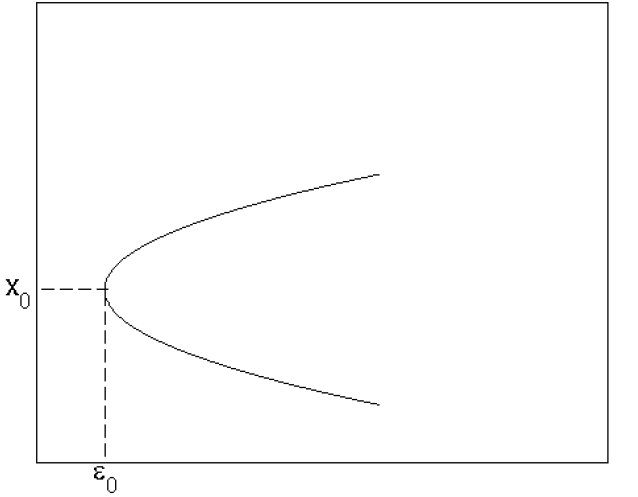
\includegraphics[width=0.5\textwidth]{img/10_01}
		\par
		{\small\((x_0, \varepsilon_0)\) — точка поворота.}
		\label{fig:10_01}
	\end{figure}
	
	\subsection{Ветвление в точках бифуркации}
	
	Для особой точки \((x_0, \varepsilon_0)\): \( f(x_0, \varepsilon_0) = 0 \), \( f_x' = f_\varepsilon' = 0 \).  
	\newline
	Разложение в ряд для близкой точки \((x_0 + \Delta x, \varepsilon_0 + \Delta \varepsilon)\):
	\begin{equation}
		\begin{aligned}
			& f(x, \varepsilon) = f_x(x_0, \varepsilon_0) + f_x'(x_0, \varepsilon_0)\Delta x + f_\varepsilon''(x_0, \varepsilon_0)\Delta \varepsilon + \\ 
			& \hspace{-2em}+ \frac{1}{2} \left( A \Delta x^2 + 2 B \Delta x \Delta \varepsilon + C \Delta \varepsilon^2 \right) + o(\|\Delta x\|^2 + \|\Delta \varepsilon\|^2),
		\end{aligned}
	\end{equation}
	Получаем
	\vspace{-1em}
	\begin{equation}
		f(x, \varepsilon) = \frac{1}{2} \left( A \Delta x^2 + 2 B \Delta x \Delta \varepsilon + C \Delta \varepsilon^2 \right) + o(\|\Delta x\|^2 + \|\Delta \varepsilon\|^2),
	\end{equation}
	\vspace{-0.5em}
	Для удобства заменим \textbf{o}-малая на (***):
	\begin{equation}
		f(x, \varepsilon) = \frac{1}{2} \left( A \Delta x^2 + 2 B \Delta x \Delta \varepsilon + C \Delta \varepsilon^2 \right) + (***),
	\end{equation}
	где \( A = f_{xx}''(x_0, \varepsilon_0) \), \( B = f_{x\varepsilon}''(x_0, \varepsilon_0) \), \( C = f_{\varepsilon\varepsilon}''(x_0, \varepsilon_0) \), 
	\newline
	(***) – слагаемые третьего и более высокого порядка малости.
	\par
	\vspace{0.5em}
	\textbf{Случай 1: \( A \neq 0 \)} \(\Rightarrow\) разделим на \(\Delta \varepsilon^2 \) и перейдем к пределу при \(\Delta \varepsilon \rightarrow\) 0.
	\newline
	Уравнение:
	\begin{equation}
		A \left( \frac{d x}{d \varepsilon} \right)^2 + 2 B \frac{d x}{d \varepsilon} + C = 0, \quad D = B^2 - A C.
	\end{equation}
	\begin{itemize}
		\item \( D < 0 \): изолированная точка.
		\vspace{-0.7em}
		\item \( D > 0 \): две пересекающиеся ветви.
	\end{itemize}
	\vspace{-1em}
	\begin{figure}[H]
		\centering
		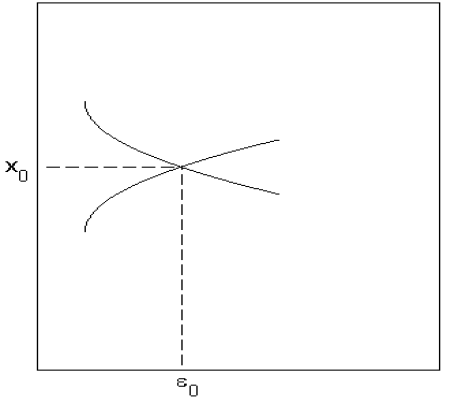
\includegraphics[width=0.35\textwidth]{img/10_02}
		\par
		{\small \((x_0, \varepsilon_0)\) — точка ветвления.}
		\label{fig:10_02}
	\end{figure}
	\vspace{-1em}
	\textbf{Случай 2: \( A = 0 \), \( C \neq 0 \)} \(\Rightarrow\) разделим на \(\Delta x^2 \) и перейдем к пределу при \(\Delta x \rightarrow\) 0.
	\newline
	Уравнение:
	\begin{equation}
		C \left( \frac{d\varepsilon}{dx} \right)^2 + 2B \frac{d\varepsilon}{dx} + A = C \left( \frac{d\varepsilon}{dx} \right)^2 + 2B \frac{d\varepsilon}{dx} = 0.
	\end{equation}
	Корни:
	\begin{equation}
		\left( \frac{d \varepsilon}{d x} \right)_1 = 0, \quad \left( \frac{d \varepsilon}{d x} \right)_2 = -\frac{2 B}{C}.
	\end{equation}
	Бифуркация типа «вилка».
	\vspace{-1em}
	\begin{figure}[H]
		\centering
		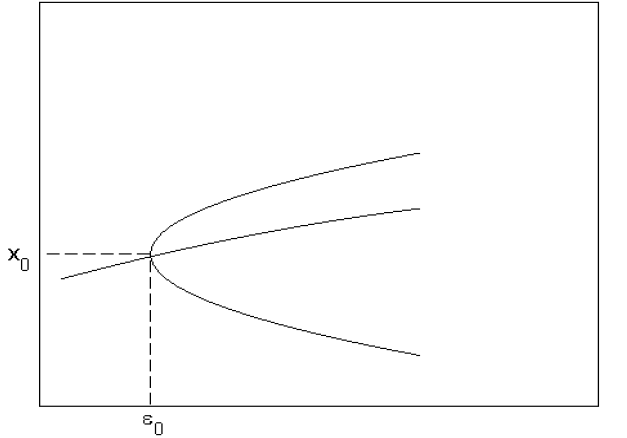
\includegraphics[width=0.35\textwidth]{img/10_03}
		\par
		{\small Бифуркация типа «вилка».}
		\label{fig:10_03}
	\end{figure}
	
	\newpage
	
	\subsection{Комплексная бифуркация (Андронова-Хопфа)}
	
	Рассмотрим систему:
	\begin{equation}
		\begin{cases}
			\frac{d x_1}{d t} = \varepsilon x_1 - x_2 \mp x_1 (x_1^2 + x_2^2), \\
			\frac{d x_2}{d t} = x_1 + \varepsilon x_2 \mp x_2 (x_1^2 + x_2^2).
		\end{cases}
	\end{equation}
	
	\textbf{Случай со знаком «минус»}
	\newline 
	Стационарная точка: \((0, 0)\). Матрица Якоби:
	\begin{equation}
		J = \begin{pmatrix} \varepsilon & -1 \\ 1 & \varepsilon \end{pmatrix}, \quad \lambda_{1,2} = \varepsilon \pm i.
	\end{equation}
	В полярных координатах (\( x_1 = R \cos \varphi \), \( x_2 = R \sin \varphi \)):
	\begin{align}
		R'\cos\varphi - R\sin\varphi \cdot \varphi' &= \varepsilon R\cos\varphi - R\sin\varphi - R^3\cos\varphi, \\
		R'\sin\varphi + R\cos\varphi \cdot \varphi' &= R\cos\varphi + \varepsilon R\sin\varphi - R^3\sin\varphi.
	\end{align}
	
	Умножим на $\cos\varphi$ и $\sin\varphi$ соответственно, и результаты сложим:
	\begin{equation}
		\frac{d R}{d t} = \varepsilon R - R^3 = R (\varepsilon - R^2), \quad \frac{d \varphi}{d t} = 1.
	\end{equation}
	Стационарные точки: \( R = 0 \), \( R = \sqrt{\varepsilon} \) (при \(\varepsilon > 0\)).  
	\begin{itemize}
		\item \(\varepsilon < 0\): устойчивый фокус (\( R \to 0 \)).
		\item \(\varepsilon = 0\): устойчивый фокус (\( R' = -R^3 < 0 \)).
		\item \(\varepsilon > 0\): неустойчивый фокус, предельный цикл \( R = \sqrt{\varepsilon} \).
	\end{itemize}
	\vspace{-1em}
	\begin{figure}[H]
		\centering
		\begin{minipage}{0.18\textwidth}
			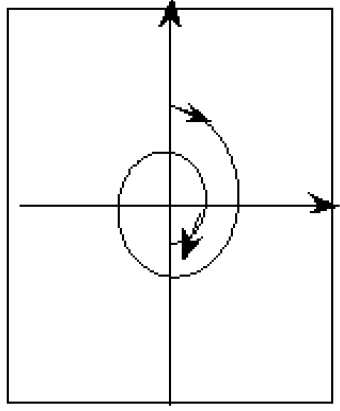
\includegraphics[width=\textwidth]{img/10_04}
			\par
			\centering{\small\(\varepsilon < 0\)}
		\end{minipage}
		\begin{minipage}{0.2\textwidth}
			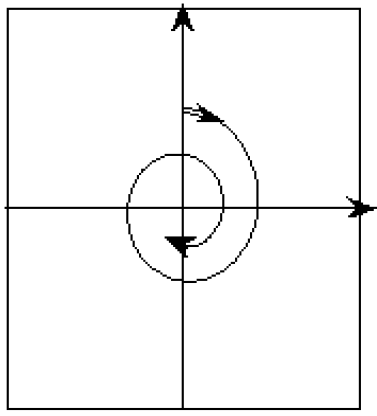
\includegraphics[width=\textwidth]{img/10_05}
			\centering{\small\(\varepsilon = 0\)}
		\end{minipage}
		\begin{minipage}{0.19\textwidth}
			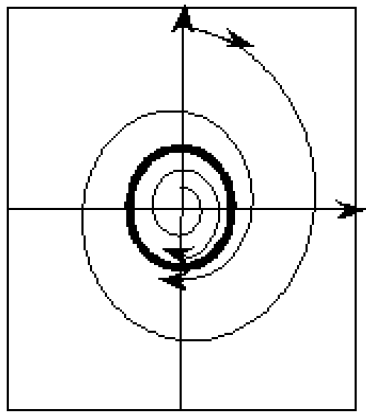
\includegraphics[width=\textwidth]{img/10_06}
			\centering{\small\(\varepsilon > 0\)}
		\end{minipage}
	\end{figure}
	\vspace{-1em}
	\textbf{Случай со знаком «плюс»}
	\newline
	Аналогичными действиями получаем:
	\begin{equation}
		\frac{d R}{d t} = \varepsilon R + R^3 = R (\varepsilon + R^2), \quad \frac{d \varphi}{d t} = 1.
	\end{equation}
	Стационарные точки: \( R = 0 \), \( R = \sqrt{-\varepsilon} \) (при \(\varepsilon < 0\)).  
	\begin{itemize}
		\item \(\varepsilon < 0\): устойчивый фокус (\( R \to 0 \) при \( R < \sqrt{-\varepsilon} \)), \( R \to \infty \) при \( R > \sqrt{-\varepsilon} \).
		\item \(\varepsilon \geq 0\): неустойчивый фокус (\( R \to \infty \))
	\end{itemize}
	\vspace{-1em}
	\begin{figure}[H]
		\centering
		\begin{minipage}{0.247\textwidth}
			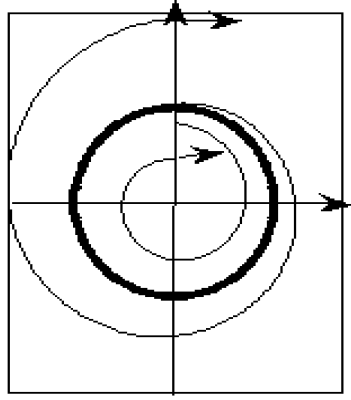
\includegraphics[width=\textwidth]{img/10_07}
			\centering{\small\(\varepsilon < 0\)}
		\end{minipage}
		\begin{minipage}{0.25\textwidth}
			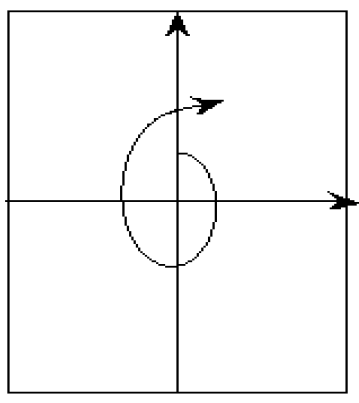
\includegraphics[width=\textwidth]{img/10_08}
			\centering{\small\(\varepsilon = 0\)}
		\end{minipage}
		\begin{minipage}{0.25\textwidth}
			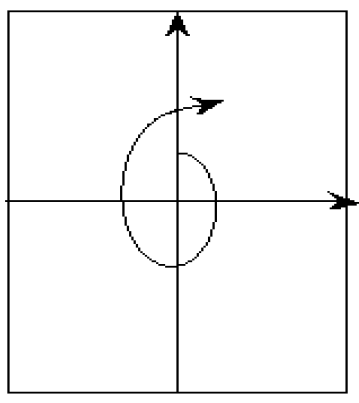
\includegraphics[width=\textwidth]{img/10_08}
			\centering{\small\(\varepsilon > 0\)}
		\end{minipage}
	\end{figure}
	
	\newpage
	
	\section {Методы получения стационарных решений. Метод продолжения по параметру}
	\subsection{Методы построения диаграмм стационарных решений}
	
	Стационарные точки системы \(\frac{d x}{d t} = f(x, \varepsilon)\):
	\begin{equation}
		f(x, \varepsilon) = 0.
	\end{equation}
	\begin{itemize}
		\item Дискретизация: \(\varepsilon_k = \varepsilon_0 + k \Delta \varepsilon\).
		\item Решаем, например, методом Ньютона с начальным приближением \(x_{k-1}\) для \(x_k\). 
		\par
		\vspace{0.5em}
		Последовательно получаем \(x_k = x(e_k)\). При этом для относительно малого шага \(\Delta e\) значение \(x_{k-1}\) будет хорошим начальным приближением, и метод Ньютона будет успешно сходиться.
		\newline
		Остается лишь вопрос с выбором удачного значения \(x_0\). Для его нахождения может быть использован следующий подход.
	\end{itemize}
	
	\subsection{Метод продолжения по параметру}
	Вместо поиска решения уравнения:
	\begin{equation}
		f(x) = f(x, \varepsilon_0) = 0
	\end{equation}
	\par
	\vspace{-0.5em}
	Решаем:
	\begin{equation}
		H(\tau, x) = 0, \quad \tau \in [0, 1],
	\end{equation}
	где \(H(0, x) = 0\) тривиально, а \(H(1, x) = f(x)\).
	\newline
	Примеры:
	\begin{equation}
		H(\tau, x) = f(x) + (\tau - 1) \cdot f(x^*),
	\end{equation}
	\begin{equation}
		H(\tau, x) = (1 - \tau) \cdot (x - x^*) + \tau \cdot f(x).
	\end{equation}
	Шаг \(\tau_j = j \cdot \Delta \tau, \Delta \tau = 1/ N, j = 0, 1, ..., N\), решение дает \(x_0\).
	\par
	\vspace{0.5em}
	Для окончательного определения параметров стационарных решений в каждой найденной точке \( x_k = x(\varepsilon_k) \) вычисляем матрицу Якоби системы и рассчитываем её собственные значения, а затем «раскрашиваем» по устойчивости кривые \( x(\varepsilon) \). Если стационарная задача определения точек вещественной или комплексной бифуркации, то здесь может быть использован следующий алгоритм.
	
	\newpage
	\section{Понятие бифуркации. Точки ветвления и поворота, бифуркация Андронова-Хопфа}
	
	\subsection{Точки поворота и ветвления}
	
	Расширяем \(x\) до \( x^{(n+1)} = \varepsilon \), матрица \(J\) размером \( n \times (n+1) \):
	\begin{equation}
		J = \begin{pmatrix}
			\frac{\partial f^{(1)}}{\partial x^{(1)}} & \cdots & \frac{\partial f^{(1)}}{\partial x^{(n+1)}} \\
			\vdots & \ddots & \vdots \\
			\frac{\partial f^{(n)}}{\partial x^{(1)}} & \cdots & \frac{\partial f^{(n)}}{\partial x^{(n+1)}}
		\end{pmatrix}.
	\end{equation}
	Пусть \(J_k\) – квадратная матрица, получившаяся из \(J\) вычеркиванием \textbf{k}-го столбца. 
	\par
	Тогда \(J_{n+1}\) — матрица Якоби. Условие бифуркации:
	\begin{equation}
		\det(J_{n+1}) = 0.
	\end{equation}
	\begin{itemize}
		\item \textit{Точка ветвления:} \(\det(J_k) = 0\) для \( k \neq n+1 \).
		\item \textit{Точка поворота:} \(\det(J_k) \neq 0\) для \( k \neq n+1 \).
	\end{itemize}
	Если размерность вектора \( x \) не мала, то формирование \(\det(J_{n+1}) = 0\) становится затруднительным. 
	\par
	Для упрощения вместо условия нулевого определителя используется уравнение \( J_{n+1} \cdot v = 0 \), 
	\par
	где \( v \) - собственный вектор, соответствующий нулевому собственному значению.
	\begin{equation}
		\begin{cases}
			f(x, \varepsilon) = 0, \\
			J_{n+1} \cdot v = 0, \\
			v^{(k)} = 1.
		\end{cases}
	\end{equation}

	\subsection{Точки комплексной бифуркации (Андронова-Хопфа)}
	
	В точке бифуркации: 
	\begin{equation}
	\lambda_{1,2} = \pm i \omega, \omega = u \pm i v.
	\end{equation}
	где \(\lambda_{1,2}\) - чисто мнимая пара собств. значений, а \(\omega\) - комплексно-сопряженная пара собств. векторов.
	\begin{equation}
		J_{n+1} w = \lambda w \implies J_{n+1} (u + i v) = \lambda (u + i v).
	\end{equation}
	Приравнивая действительные и мнимые части отдельно, имеем:
	\begin{equation}
		J_{n+1} \cdot u + \omega \cdot v = 0, \quad -\omega \cdot u + J_{n+1} \cdot v = 0.
	\end{equation}
	\par
	Дополняя условием нормировки, получаем систему из (3n+2) уравнений:
	\begin{equation}
		\begin{cases}
			f(x, \varepsilon) = 0, \\
			J_{n+1} \cdot u + \omega \cdot v = 0, \\
			-\omega \cdot u + J_{n+1} \cdot v = 0, \\
			u^{(k)} = 1, \quad v^{(k)} = 0.
		\end{cases}
	\end{equation}
	
	Для \( n = 2 \):
	\begin{equation}
		J_{n+1} = \begin{pmatrix} a_{11} & a_{12} \\ a_{21} & a_{22} \end{pmatrix}, \quad \lambda_{11} + \lambda_{22} = a_{11} + a_{22} = 0.
	\end{equation}
	Решаем:
	\begin{equation}
		\begin{cases}
			f(x, \varepsilon) = 0, \\
			a_{11} + a_{22} = 0,
		\end{cases}
	\end{equation}
	с проверкой типа \(\lambda\).
	
	\newpage
	
	% ЁПТАААААААААААААААААААААААААААААААААААААААААААААААААААААААААААА
	\section{Получение периодического решения, его орбитальная устойчивость}
	% Нахождение периодического решения
	\subsection{Получение периодического решения}
	\textbf{Проблема} применения традиционных методов — неопределённость промежутка интегрирования T.
	\par
	Для поиска периодического решения системы
	\begin{equation}
		\frac{d x}{d t} = f(x), \quad x(T) = x(0),
	\end{equation}
	с неизвестным \( T \) выполним замену \( t = T \tau \):
	\begin{equation}
		\frac{d x}{d \tau} = T f(x), \quad x(1) = x(0), \quad \tau \in [0,1].
	\end{equation}
	Здесь \( n \) уравнений \( x(1) = x(0) \) определяют \( n+1 \) неизвестное (\( x(0) \) и \( T \)). 
	\par
	\textbf{Неоднозначность}: возможность выбора любой точки траектории периодического решения в качестве начальной. Поэтому фиксируем одну компоненту, например, \( x^{(j)}(0) = \alpha \).
	
	\subsection{Оценка орбитальной устойчивости}
	Для устойчивости вычисляем \textbf{матрицу монодромии} \( U(1) \) и находим её мультипликаторы.
	\par
	\(x(\tau) = U(\tau) x(0)\), для элементов \(u_{ik} (\tau)\) матрицы \(U(\tau)\) получаем:
	\begin{equation}
		u_{ik}(\tau) = \frac{\partial x^{(i)}(\tau)}{\partial x^{(k)}(0)}
	\end{equation} 
	Они удовлетворяют
	\begin{equation}
		\frac{d u_{ik}(\tau)}{dt} = T \cdot \sum_{s=1}^{n} \frac{\partial f^{(i)}}{\partial x^{(s)}} u_{sk}(\tau), 
		\quad u_{ik}(0) = 
		\begin{cases}
			0, & i \ne k \\
			1, & i = k
		\end{cases}.
	\end{equation}
	Эта система решается совместно с уравнением \(\frac{d x}{d t} = f(x)\), в результате чего получается матрица \(U(1)\), мультипликаторы которой характеризуют орбитальную устойчивость периодич. решения.
	
	\newpage
	
	\section{Виды бифуркации периодического решения. Отображение Пуанкаре, алгоритмы его построения}
	% Виды бифуркаций
	\subsection{Виды бифуркации периодического решения}
	
	При изменении параметра \( \varepsilon \) возможны бифуркации:
	
	\begin{enumerate}
		\item \textbf{Рождение пары циклов.} Появляется второй мультипликатор \( \rho = 1 \).
		\begin{figure}[H]
			\centering
			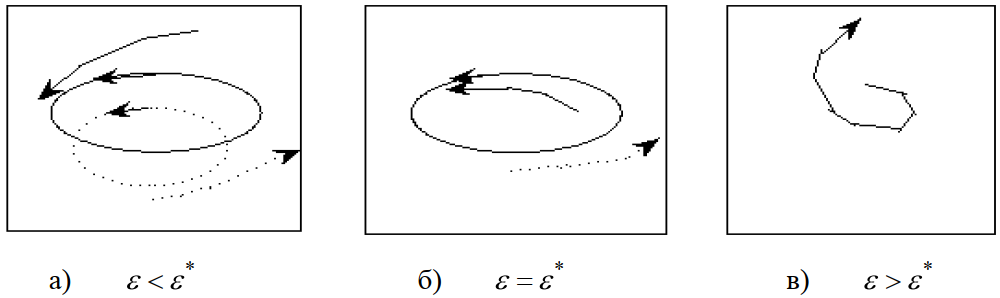
\includegraphics[width=1\linewidth, height=0.15\textheight]{img/14_01}
			{\small Исчезновение пары замкнутых траекторий}
			\label{fig:14_01}
		\end{figure}
		\vspace{-1em}
		\item \textbf{Удвоение периода.} Один мультипликатор становится \( \rho = -1 \).
		\begin{figure}[H]
			\centering
			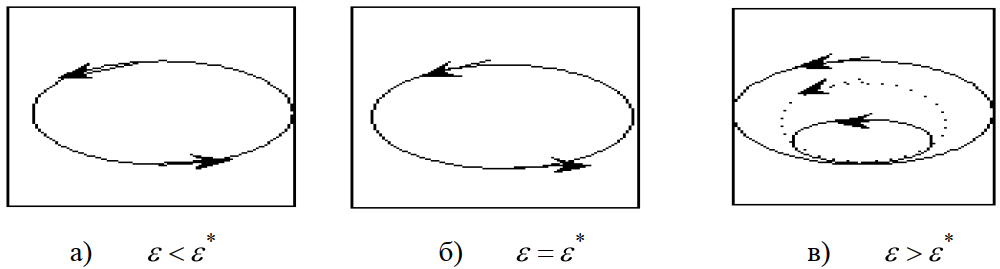
\includegraphics[width=1\linewidth, height=0.15\textheight]{img/14_02}
			{\small Бифуркация удвоения периода}
			\label{fig:14_02}
		\end{figure}
		\vspace{-1em}
		\item \textbf{Возникновение тора.} Пара комплексных мультипликаторов достигает \( |\rho| = 1 \).
		\begin{figure}[H]
			\centering
			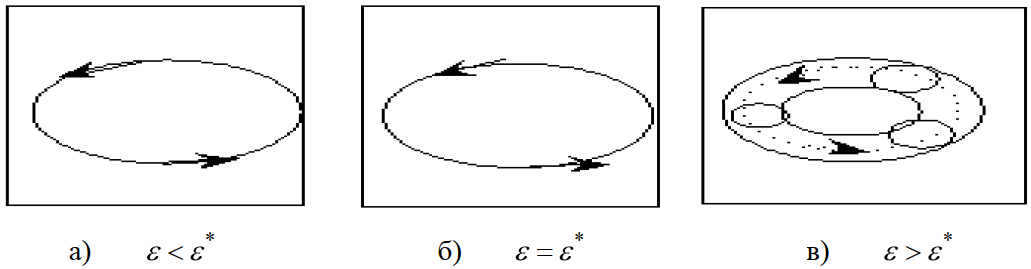
\includegraphics[width=1\linewidth, height=0.15\textheight]{img/14_03}
			{\small Возникновение инвариантного тора}
			\label{fig:14_03}
		\end{figure}
	\end{enumerate}
	\vspace{-2em}
	% Отображение Пуанкаре
	
	\subsection{Отображение Пуанкаре}
	
	\subsubsection{Определение отображения Пуанкаре}
	
	Основная идея:
	\begin{itemize}
		\item Пусть \(\gamma(x_0)\) — замкнутая траектория решения системы
		\begin{equation}
			\frac{dx}{dt} = f(x), \quad x \in \mathbb{R}^n,
		\end{equation}
		\item Выберем точку \(x_0 \in \gamma\) и проведем через нее сечение \(\Sigma\) — часть гиперплоскости, пересекающей \(\gamma\) под ненулевым углом.
		\item Траектории, близкие к \(\gamma\), задают отображение Пуанкаре \(P: \Sigma \to \Sigma\), где \(P(x_0)\) — первая точка пересечения траектории \(\gamma(x_0)\) с \(\Sigma\) после \(x_0\).
		
		\begin{equation}
			x_1 = P(x_0), \quad x_2 = P(x_1), \quad \dots, \quad x_k = P^k(x_0).
		\end{equation}
	\end{itemize}
	
	Характеристики отображения:
	\begin{itemize}
		\item Предельному циклу соответствует неподвижная точка \(x_0 \in \Sigma\): \(P(x_0) = x_0\).
		\item Бифуркация рождения (исчезновения) пары замкнутых траекторий связана с появлением двух неподвижных точек.
		\item Бифуркация удвоения периода соответствует траектории, замыкающейся после двух обходов: \(x_1 = P(x_0)\), \(x_0 = P(x_1)\).
		\item Возникновение инвариантного тора сопровождается ответвлением замкнутой инвариантной кривой отображения \(P\).
	\end{itemize}
	\vspace{-1em}
	\begin{figure}[H]
		\centering
		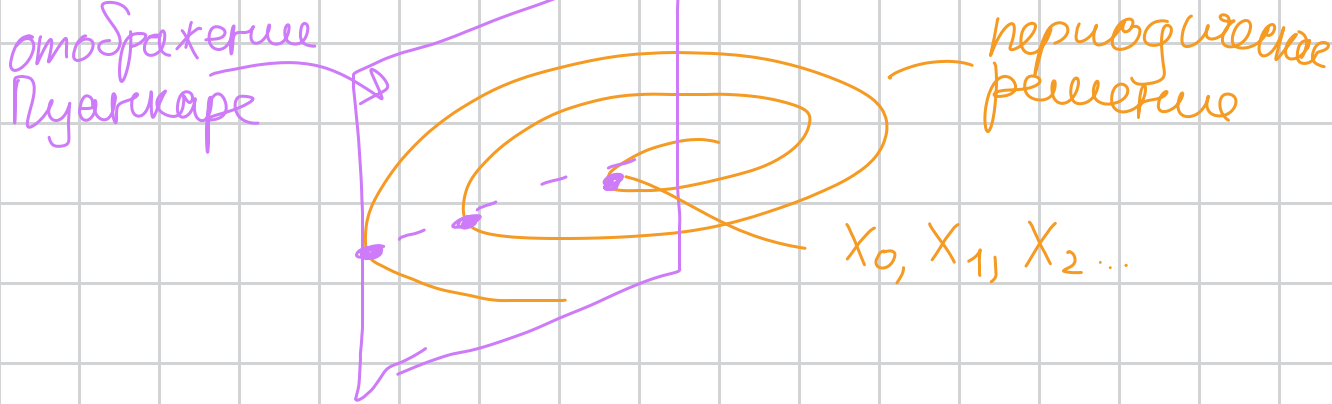
\includegraphics[width=1\linewidth, height=0.15\textheight]{img/14_04}
		\label{fig:14_04}
	\end{figure}
	\vspace{-2em}
	Преимущества отображения Пуанкаре:
	\begin{itemize}
		\item Снижение размерности системы на единицу (работа в сечении \(\Sigma\)).
		\item Дискретизация времени: дифференциальные уравнения заменяются разностными.
		\item Сокращение объема данных, так как учитываются только точки пересечения с \(\Sigma\).
	\end{itemize}
	
	\subsubsection{Алгоритм построения отображения Пуанкаре}
	
	1) Долгий грустный обычный вариант:
	\begin{itemize}
		\item Сечение \(\Sigma\) задается уравнением гиперповерхности
		\begin{equation}
			S(x) = S(x^{(1)}, x^{(2)}, \dots, x^{(n)}) = 0,
		\end{equation}
		где \(S(x)\) — скалярная функция, определяющая сечение.
		\item Стандартный метод нахождения точек пересечения траектории с \(\Sigma\) основан на численном интегрировании системы
		\begin{equation}
			\frac{dx}{dt} = f(x).
		\end{equation}
		\item При смене знака \(S(x)\) м/у двумя соседними точками, напр., \(S(x(t_m)) < 0\), \(S(x(t_{m+1})) > 0\), выполняется итерационное уточнение шага на \([t_m, t_{m+1}]\), чтобы \(S(x) = 0\) с зад. точностью. 
		\par
		Этот процесс повторяется для каждой т. пересечения, что требует значительных вычислений.
	\end{itemize}
	\newpage
	2) Модифицированный оптимизированный алгоритм:
	\begin{itemize}
		\item Сечение \(\Sigma\) задается уравнением
		\begin{equation}
			S(x) = x^{(k)} - a = 0,
		\end{equation}
		где \(x^{(k)}\) — \(k\)-я компонента вектора \(x\), \(a\) — константа. 
		\item Перейдем к независимой переменной \(x^{(k)}\) вместо \(t\). Тогда система преобразуется в
		\begin{equation}
			\frac{dx^{(i)}}{dx^{(k)}} = \frac{f^{(i)}(x)}{f^{(k)}(x)}, \quad i \neq k,
		\end{equation}
		\begin{equation}
			\frac{dt}{dx^{(k)}} = \frac{1}{f^{(k)}(x)},
		\end{equation}
		где \(f^{(i)}(x)\) — \(i\)-я компонента \(f(x)\).
		
		\item Достигнув точки \(x(t_m)\), выполняем шаг интегрирования по \(x^{(k)}\) размером \(\Delta x^{(k)} = a - x^{(k)}(t_m)\), чтобы сразу попасть на \(\Sigma\).
		
		\item Далее продолжим интегрирование системы в обычном виде \(\frac{dx}{dt} = f(x).\)
		
		\item Если сечение задано общим уравнением \(S(x^{(1)}, x^{(2)}, \dots, x^{(n)}) = 0\), 
		\par
		расширяем вектор \(x\), добавляя компоненту
		\begin{equation}
			x^{(n+1)} = S(x^{(1)}, x^{(2)}, \dots, x^{(n)}),
		\end{equation}
		и дополняем систему уравнением
		\begin{equation}
			\frac{dx^{(n+1)}}{dt} = \sum_{j=1}^n \frac{\partial S}{\partial x^{(j)}} \cdot f^{(j)}(x).
		\end{equation}
		
		Тогда сечение упрощается до \(x^{(n+1)} = 0\),
		\par
		что сводит задачу к случаю \(S(x) = x^{(k)} - a = 0\).
	
	\end{itemize}
	
	\section{Построение бифуркационных диаграмм для периодических решений. Структурная схема анализа нелинейных моделей}
	
	\subsection{Нахождение точек бифуркации}
	
	Рассмотрим систему \(\frac{d x}{d t} = f(x)\), введя в нее скалярный параметр \(\varepsilon\):
	\begin{equation}
		\frac{dx}{d\tau} = T \cdot f(x, \varepsilon), \quad x(1) = x(0), \quad \tau \in [0,1],
	\end{equation}
	где \(T\) — период, \(\tau = t/T\) — нормированное время. 
	\par
	Система решается совместно с уравнениями для матрицы монодромии \(U(\tau)\):
	\begin{equation}
		\frac{du_{ik}(\tau)}{d\tau} = T \cdot \sum_{s=1}^n \frac{\partial f^{(i)}}{\partial x^{(s)}} u_{sk}(\tau), \quad u_{ik}(0) = \begin{cases} 
			0, & i \neq k, \\
			1, & i = k,
		\end{cases}
	\end{equation}
	где \(u_{ik}(\tau) = \frac{\partial x^{(i)}(\tau)}{\partial x^{(k)}(0)}\) — элементы матрицы \(U(\tau)\).
	
	Мультипликаторы матрицы \(U(1)\) определяют орбитальную устойчивость.
	\par
	Далее нужны доп.условия для определения \(\varepsilon\)
	\newpage
	\subsubsection{Бифуркация удвоения периода.} 
	\vspace{-0.5em}
	Один из мультипликаторов \(U(1)\) равен \(-1\). Для собственного вектора \(v\):
	\begin{equation}
		(U(1) + E) \cdot v = 0, \quad v^{(k)} = 1,
	\end{equation}
	где \(E\) — ед. матрица, \(v^{(k)}\) - \(k\)-я компонента \(v\). Это дает \(n+1\) ур-ий для \(n+1\) неизвестных (\(v\), \(\varepsilon\)).
	\vspace{-1em}
	\subsubsection{Рождение (исчезновение) пары замкнутых траекторий.}
	\vspace{-0.5em}
	Появляется мультипликатор, равный 1. Возможны два случая:
	\begin{enumerate}[leftmargin=1.4em] % уменьшение отступа между пунктами
		\item Два линейно независимых собственных вектора \(v\) и \(w\):
		\vspace{-0.5em}
		\begin{equation}
			\begin{aligned}
				&(U(1) - E) \cdot v = 0, \\
				&(U(1) - E) \cdot w = 0.
			\end{aligned}
			\vspace{-0.5em}
		\end{equation}
		\item Один собственный вектор \(v\) и один корневой вектор \(w\):
		\vspace{-0.5em}
		\begin{equation}
			\begin{aligned}
				&(U(1) - E) \cdot v = 0, \\
				&(U(1) - E) \cdot w = v.
			\end{aligned}
			\vspace{-0.5em}
		\end{equation}
		Для учета обеих ситуаций:
		\vspace{-0.25em}
		\begin{equation}
			\begin{aligned}
				&(U(1) - E) \cdot v = 0, \\
				&(U(1) - E)^2 \cdot w = 0, \\
				&v^{(k)} = 1, \quad w^{(k)} = 0.
			\end{aligned}
			\vspace{-0.5em}
		\end{equation}
	\end{enumerate}
	\vspace{-1.75em}
	\subsubsection{Возникновение инвариантного тора.} 
	Модуль комплексно-сопряженной пары мультипликаторов \(\lambda_{1,2} = \alpha \pm i \omega\) равен 1. 
	\par
	Для собственных векторов \(u \pm i v\):
	\vspace{-0.5em}
	\begin{equation}
		U(1) \cdot (u + i v) = (\alpha + i \omega) \cdot (u + i v).
	\end{equation}
	\vspace{-0.5em}
	Разделяя действительную и мнимую части:
	\begin{equation}
		\begin{aligned}
			&(U(1) - \alpha E) \cdot u + \omega \cdot v = 0, \\
			&-\omega \cdot u + (U(1) - \alpha E) \cdot v = 0, \\
			&u^{(k)} = 1, \quad v^{(k)} = 0, \\
			&\alpha^2 + \omega^2 = 1.
		\end{aligned}
		\vspace{-0.5em}
	\end{equation}
	Решение систем для мультипликаторов совместно с уравнениями для \(U(\tau)\) позволяет строить 
	\par
	бифуркационные диаграммы, варьируя \(\varepsilon\).
	\vspace{-1.25em}
	\subsection{Структурная схема анализа нелинейных моделей}
	\vspace{-1.5em}
	\begin{figure}[H]
		\centering
		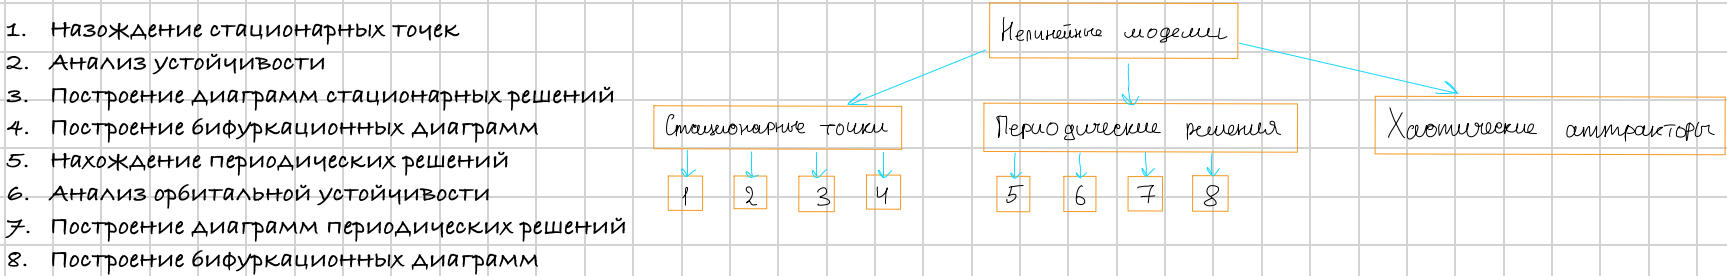
\includegraphics[width=1\linewidth, height=0.15\textheight]{img/15_01}
		\label{fig:15_01}
	\end{figure}
	\vspace{-2em}
	% Итоги и задачи
	\subsection{Используемый мат.аппарат}
	\vspace{-1.5em}
	\begin{figure}[H]
		\centering
		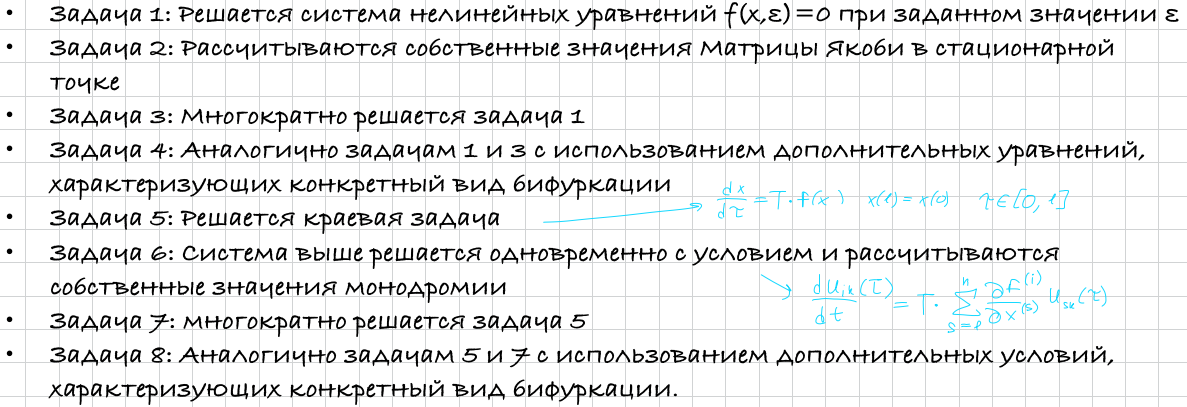
\includegraphics[width=1\linewidth, height=0.15\textheight]{img/15_02}
		\label{fig:15_02}
	\end{figure}
	
	\newpage
	
	\section{Понятие аттрактора. Странные аттракторы, пример механизма их возникновения (явление Фейгенбаума, субгармонический каскад)}
	
	\subsection{Определения}
	
	% Описываем базовую систему уравнений
	Рассмотрим систему нелинейных дифференциальных уравнений:
	\begin{equation}
		\frac{d x}{d t} = f(x), \quad x \in \mathbb{R}^n,
	\end{equation}
	где $x$ — вектор состояния, $f(x)$ — нелинейная функция.
	\par
	\vspace{0.5em}
	% Вводим ключевые определения
	\textbf{\textit{\uline{DEF 1.}}} Множество $M \subset \mathbb{R}^n$ называется \textbf{инвариантным множеством} системы, если любая траектория решения, пересекающая $M$, целиком содержится в $M$. 
	\par
	\textit{Примеры}: стационарные точки, предельные циклы.
	\par
	\vspace{0.5em}
	\textbf{\textit{\uline{DEF 2.}}} Замкнутое инвариантное множ. $M$ реш. $x(t)$ называется \textbf{устойчивым по Ляпунову}, если:
	\begin{equation}
		(\forall \varepsilon > 0)(\exists \delta \in (0, \varepsilon))(\forall t \geq 0) \left( \rho(x_0, M) \leq \delta \Rightarrow \rho(x, M) \leq \varepsilon \right),
	\end{equation}
	где $\rho$ — расстояние от точки до множества.
	\par
	\vspace{0.5em}
	\textbf{\textit{\uline{DEF 3.}}} Замкнутое инвариантное множество $\textgoth{A}$ называется \textbf{аттрактором}, если существует открытое множество $U$, такое что $\textgoth{A} \subset U$ и:
	\begin{equation}
		(\forall x_0 \in U) \left( \rho(x, \textgoth{A}) \to 0 \quad \text{при} \quad t \to \infty \right).
	\end{equation}
	При этом $U$ — область притяжения аттрактора $\textgoth{A}$.
	\par
	\vspace{0.5em}
	\textbf{\textit{\uline{DEF 4.}}} Инвариантное множество $M$ называется \textbf{внутренне неустойчивым (хаотическим)}, если траектории в $M$ неустойчивы по Ляпунову, а близкие траектории расходятся экспоненциально.
	
	\subsection{Явление Фейгенбаума}
	
	% Вводим разностное уравнение
	Рассмотрим разностное уравнение:
	\begin{equation}
		x_{k+1} = f(x_k), \quad f(x) = 4\varepsilon x (1 - x), \quad x \in [0,1], \quad \varepsilon \in [0,1],
	\end{equation}
	где $\varepsilon$ — параметр. максимум функции:
	\begin{equation}
		\max f(x) = f\left(\frac{1}{2}\right) = \varepsilon.
	\end{equation}
	Значения $x_k$ остаются в $[0,1]$.
	
	% Стационарные точки
	Стационарные точки уравнения $f(x) = 4\varepsilon x (1 - x)$:
	\begin{equation}
		x_1^{\text{ст}} = 0, \quad x_2^{\text{ст}} = 1 - \frac{1}{4\varepsilon}.
	\end{equation}
	
	\newpage
	
	% Анализ устойчивости для разных интервалов epsilon
	Проанализируем поведение системы:
	
	\textbf{Промежуток 1.} $\varepsilon \in [0, 0.25)$. Точка $x_2^{\text{ст}}$ вне $[0,1]$. Устойчивость $x_1^{\text{ст}} = 0$:
	\begin{equation}
		f'(x) = 4\varepsilon - 8\varepsilon x, \quad f'(0) = 4\varepsilon < 1 \quad (\varepsilon < 0.25).
	\end{equation}
	Решения $x_k \to 0$ для всех $x_0$.
	
	\textbf{Промежуток 2.} $\varepsilon \in [0.25, 0.75)$. Точка $x_1^{\text{ст}} = 0$ неустойчива, $x_2^{\text{ст}}$ устойчива:
	\begin{equation}
		f'(x_2^{\text{ст}}) = 4\varepsilon - 8\varepsilon x_2^{\text{ст}} = 4\varepsilon - 8\varepsilon \left(1 - \frac{1}{4\varepsilon}\right) = 2 - 4\varepsilon, \quad |f'(x_2^{\text{ст}})| \leq 1.
	\end{equation}
	Решения сходятся к $x_2^{\text{ст}}$.
	
	\textbf{Промежуток 3.} $\varepsilon \in [0.75, 0.86237\ldots)$. Обе точки неустойчивы, появляется аттрактор периода 2:
	\begin{equation}
		x_2^* = f(x_1^*), \quad x_1^* = f(x_2^*).
	\end{equation}
	
	\textbf{Промежуток 4.} $\varepsilon \in [0.86237\ldots, 0.88602\ldots)$. Аттрактор пер.2 неустойчив, появл.аттрактор пер.4:
	\begin{equation}
		x_2^{**} = f(x_1^{**}), \quad x_3^{**} = f(x_2^{**}), \quad x_4^{**} = f(x_3^{**}), \quad x_1^{**} = f(x_4^{**}).
	\end{equation}
	
	\textbf{Промежуток 5.} $\varepsilon \in [0.88602\ldots, 0.89218\ldots)$. Аттрактор пер.4 неустойчив, появл.аттрактор пер.8.
	
	% Описание каскада удвоения периода
	Процесс удв. периода продолжается до $\varepsilon_\infty=0.892486\ldots$, с коэф. сжатия интервалов $\delta=4.6692016\ldots$
	
	\subsection{Субгармонический каскад}
	
	\begin{itemize}
		\item В результате последовательной бифуркации удвоения периода 
		\textbf{субгармонический каскад} возникают хаотические аттракторы.
		
		\item Значения \( \varepsilon > \varepsilon_{\infty} \) характеризуются сочетанием периодического аттрактора с режимом, который называют \textbf{хаосом}.
		
		\item В последнем случае \( x_k \) порождаются так, что они не повторяются, зависят от \( x_0 \), и две первоначально близкие точки порождают траектории, расходящиеся друг от друга.
		
		\item Принципиальная непредсказуемость хаотического режима при \( \varepsilon > \varepsilon_{\infty} \) не говорит об отсутствии порядка в нём - порядок просто не виден.
		
		\item \textbf{Фрактальная размерность} - одна из характеристик хаотического аттрактора.
	\end{itemize}
	
	\newpage
	
	\section{Фрактальные размерности. Аттрактор Лоренца}
	
	\subsection{Фрактальные размерности}
	
	% Определение фрактальной размерности
	Для множества в $\mathbb{R}^n$ пусть $N(\varepsilon)$ - минимальное число гиперкубов с ребром $\varepsilon$ для покрытия множ-ва. 
	\par
	\textbf{Фрактальная размерность Хаусдорфа-Безиковича}  $D$:
	\begin{equation}
		D = \lim_{\varepsilon \to 0} \frac{\ln N(\varepsilon)}{\ln (1 / \varepsilon)},
	\end{equation}
	если предел существует.
	
	% Примеры размерностей
	\textbf{Пример 1.} Точка: $N(\varepsilon) = 1 \Rightarrow D = 0$.
	
	\textbf{Пример 2.} Отрезок длины $L$: $N(\varepsilon) = \frac{L}{\varepsilon} \Rightarrow D = 1$.
	
	\textbf{Пример 3.} Поверхность площадью $S$: $N(\varepsilon) = \frac{S}{\varepsilon^2} \Rightarrow D = 2$.
	
	\textbf{Пример 4.} Канторово множество: $\varepsilon = \left(\frac{1}{3}\right)^m \Rightarrow N(\varepsilon) = 2^m$,
	\begin{equation}
		D = \lim_{m \to \infty} \frac{\ln 2^m}{\ln 3^m} = \frac{\ln 2}{\ln 3} \approx 0.63.
	\end{equation}
	
	\textbf{Пример 5.} Кривая Коха (снежинка): $\varepsilon = \left(\frac{1}{3}\right)^m \Rightarrow N(\varepsilon) = 3 \cdot 4^m$,
	\begin{equation}
		D = \lim_{m \to \infty} \frac{\ln (3 \cdot 4^m)}{\ln 3^m} = \frac{\ln 4}{\ln 3} \approx 1.26.
	\end{equation}
	
	\begin{itemize}
		\item Кривая Коха имеет свойство сечений Пуанкаре для многих хаотических аттракторов: бесконечный периметр, ограниченная конечная область плоскости.
		
		\item Исходная фигура — равносторонний $\triangle$ с единичной стороной.
		
		\item На каждом шаге: каждую сторону разделяем на 3 равные части и заменяем средний интервал равносторонним $\triangle$ без этого сегмента.
		
		\item В результате — ломаная из 4-х звеньев длины $\frac{1}{3}$, потом опять, увеличив периметр в $\frac{4}{3}$ раза и т.д.
		
		\item Предельная кривая и есть кривая Коха.
	\end{itemize}
	
	\vspace{-2em}
	\begin{figure}[H]
		\centering
		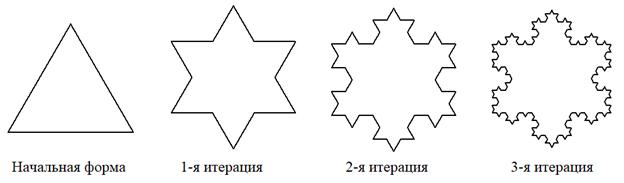
\includegraphics[width=1\linewidth, height=0.15\textheight]{img/17_01}
		\label{fig:17_01}
	\end{figure}
	\vspace{-3em}
	
	\subsection{Аттрактор Лоренца}
	
	% Система уравнений Лоренца
	Модель Лоренца описывает конвекцию:
	\begin{align}
		\frac{d x}{d t} &= \sigma (y - x), \\
		\frac{d y}{d t} &= -x z + r x - y, \\
		\frac{d z}{d t} &= x y - b z,
	\end{align}
	где $\sigma, r, b$ — параметры.
	\newpage
	% Стационарные точки и устойчивость
	Приравняв к 0 производные модели Лоренца, получим 3 стационарные точки:
	\par
	Первая: $x = y = z = 0$. Тогда матрица Якоби:
	\begin{equation}
		J = \begin{pmatrix}
			-\sigma & \sigma & 0 \\
			r - z & -1 & -x \\
			y & x & -b
		\end{pmatrix},
	\end{equation}
	в точке $(0,0,0)$:
	\begin{equation}
		J(0) = \begin{pmatrix}
			-\sigma & \sigma & 0 \\
			r & -1 & 0 \\
			0 & 0 & -b
		\end{pmatrix}.
	\end{equation}
	Характеристическое уравнение:
	\begin{equation}
		\det(J(0) - \lambda E) = (-b - \lambda) \left( \lambda^2 + (\sigma + 1) \lambda + \sigma - \sigma r \right) = 0.
	\end{equation}
	При $r < 1$ нулевая точка устойчива, при $r > 1$ — неустойчива.
	
	Вторая и третья точки (симметричные):
	\begin{equation}
		x = y = \pm \sqrt{(r - 1) b}, \quad z = r - 1,
	\end{equation}
	существуют при $r > 1$. Характеристическое уравнение:
	\begin{equation}
		\det(J - \lambda E) = -\left( \lambda^3 + (\sigma + b + 1) \lambda^2 + b (r + \sigma) \lambda + 2 \sigma b (r - 1) \right) = 0.
	\end{equation}
	
	% Условие бифуркации
	Условие комплексной бифуркации:
	\begin{equation}
		(\sigma + b + 1) b (r + \sigma) = 2 \sigma b (r - 1),
	\end{equation}
	откуда:
	\begin{equation}
		r = \frac{\sigma (\sigma + b + 3)}{\sigma - b - 1}.
	\end{equation}
	Для $\sigma = 10$, $b = \frac{8}{3}$: $r \approx 24.74$.
	% Описание поведения системы
	При $r \in [24.06, 24.74]$ — три аттрактора (две точки и хаотический).
	\par
	При $r \in (24.74, 30.1)$ — хаотический аттрактор, $D = 2.06$. 
	\par
	При $r > 30.1$ — чередование хаоса и периодичности.
	
	\newpage
	
	\section{Компонентные и топологические уравнения на макроуровне}
	
	\subsection{Метод прямой аналогии}
	% Описание метода прямой аналогии
	Метод прямой аналогии моделирует системы через подсистемы с фазовыми переменными.
	\par
	Систему делят на физич. однор. подсистемы (электрич., механич. и др.), описыв. узлами и ветвями.
	
	% Основные положения
	\begin{enumerate}
		\item Система - сумма подсистем, каждая из которых однородна.
		\item Фазовые переменные 2-х типов: потока и потенциала, а для макроуровня еще дискретизация пространства \(\Rightarrow\) \uline{конечность} множеств фазовых переменных в каждой подсистеме.
		\item Структура: узлы (вершины) и ветви (рёбра).
		\item Компонентные уравнения связывают переменные элементов через мат.модели кажд. элемента.
		\item Топологические уравнения связывают переменные взаимосвязанных элементов.
		\item[$\bullet$] Полная мат.модель - совокупность компонентных и топологических уравнений.
	\end{enumerate}
	
	% Типы элементов
	\textbf{Типы элементов:}
	\begin{itemize}
		\item $R$ — диссипация энергии (преобразование в тепло).
		\item $C$ — накопление потенциальной энергии.
		\item $L$ — накопление кинетической энергии.
	\end{itemize}
	\vspace{-1em}
	% Таблица компонентных уравнений
	\begin{figure}[H]
		\centering
		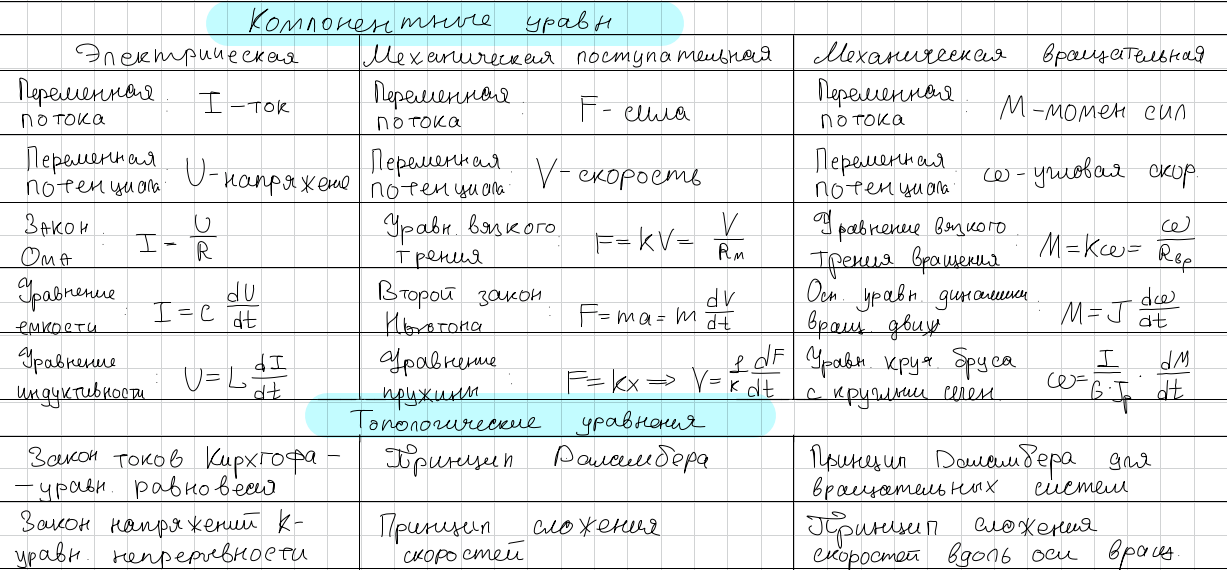
\includegraphics[width=1\linewidth, height=0.25\textheight]{img/18_01}
		\label{fig:18_01}
	\end{figure}
	
	\newpage
	
	\section{Автоматизация построения математического описания. Свойства матрицы инциденций}
	
	\subsection{Программа анализа математических моделей}
	
	% Блоки программы
	Программа состоит из четырёх блоков:
	\begin{enumerate}
		\item \textbf{Входной блок}: специальный язык описания схемы, структура данных \par
		(тип двухполюсника (ребра), узлы, номинал, начальные условия: $U_C(0)$, $I_L(0)$).
		\item \textbf{Блок построения уравнений}: использует компонентные и топологические уравнения.
		\item \textbf{Блок численной реализации}: численные методы решения.
		\item \textbf{Выходной блок}: таблицы, графики.
	\end{enumerate}
	
	\textbf{Пример модели:} Электрическая схема
	\par
	\textbf{Состав модели:}
	\vspace{-1em}
	\begin{itemize}
		\item \textbf{E} - источник напряжения
		\vspace{-1em}
		\item \textbf{I} - источник тока
		\vspace{-1em}
		\item \textbf{C} - ёмкость
		\vspace{-1em}
		\item \textbf{R} - сопротивления
		\vspace{-1em}
		\item \textbf{L} - индуктивность
		\vspace{-1em}
		\item \textbf{N} - нелинейные элементы
	\end{itemize}
	\vspace{-0.5em}
	\textbf{Граф} – множество вершин
	\par
	\textbf{Ребро} – двухполюсник
	\par
	\textbf{Вершина} – место соединения соседних элементов
	\par
	\vspace{0.5em}
	\textbf{*} Нам интересен блоĸ построения уравнений модели
	
	\vspace{-1em}
	
	\subsection{Матрица инциденций}
	
	% Описание матрицы
	Матрица $A$ строится для узлов (кроме базового) и двухполюсников.
	\begin{figure}[H]
		\centering
		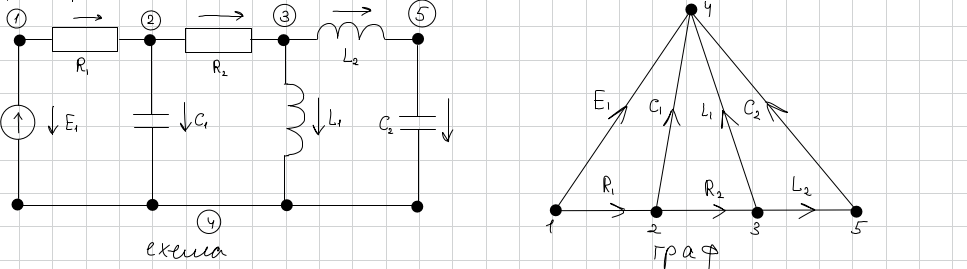
\includegraphics[width=1\linewidth, height=0.2\textheight]{img/19_01}
		\label{fig:19_01}
	\end{figure}
	\vspace{-3em}
	\hspace{-2em}
	\begin{minipage}[c][5cm][c]{0.45\textwidth} % фиксируем высоту, выравнивание по центру
		\[
		a_{ij} = 
		\begin{cases} 
			1, &- \text{узел $i$ - входной для двухполюсника $j$} \\ 
			-1, &- \text{узел $i$ - выходной для двухполюсника $j$} \\ 
			0, &- \text{иначе}
		\end{cases}
		\]
	\end{minipage}
	\hfill
	\begin{minipage}[c][5cm][c]{0.5\textwidth} % та же высота, центрирование
		\centering
		{\small Матрица инциденций для схемы\vspace{0.5em}}
		\begin{tabular}{|c|c|c|c|c|c|c|c|}
			\hline
			Узел & $E_1$ & $C_1$ & $C_2$ & $R_1$ & $R_2$ & $L_1$ & $L_2$ \\
			\hline
			1 & 1 & 0 & 0 & 1 & 0 & 0 & 0 \\
			2 & 0 & 1 & 0 & -1 & 1 & 0 & 0 \\
			3 & 0 & 0 & 0 & 0 & -1 & 1 & 1 \\
			5 & 0 & 0 & 1 & 0 & 0 & 0 & -1 \\
			\hline
		\end{tabular}
	\end{minipage}
	
	Пусть узел схемы - базовый, строки - все остальные узлы, а столбцы - двухполюсники схемы
	
	\newpage
	
	% Векторы
	Введём 3 вектора: 
	\begin{itemize}
		\item токи \(I = (i_{E_1}, i_{C_1}, i_{C_2}, i_{R_1}, i_{R_1}, i_{R_2}, i_{L_1}, i_{L_2})^T\), 
		\item напряжения \(U = (u_{E_1}, u_{C_1}, u_{C_2}, u_{R_1}, u_{R_2}, u_{L_1}, u_{L_2})^T\),
		\item потенциалы \(\varphi = (\varphi_1, \varphi_2, \varphi_3, \varphi_5)^T\).
	\end{itemize}
	В общем случае:
	\[
	\begin{cases} 
		A I = 0 - \text{закон Кирхгофа}\\ 
		U = A^T\varphi - \text{связь напряжения с потенциалом}
	\end{cases}
	\]

	\subsection{Компонентные уравнения в матрично-векторном виде}
	Двухполюсники запишем в таком порядке: $C$, $R$, $L$, $N$
	\par
	$\bullet$ \textbf{Нелинейный элемент} - независимый источник тока, управляемый источник или двухполюсник 
	\par
	с заданной вольт-амперной характеристикой:
	\[
		i_N = f_N(\varphi_i - \varphi_k)
	\]
	Тогда:
	\begin{equation}
		\begin{array}{c}
			U = (U_C,\ U_R,\ U_L,\ U_N)
			\vspace{0.5em} \\
			I = (I_C,\ I_R,\ I_L,\ I_N)
		\end{array}
		\qquad
		\Rightarrow
		\qquad
		A = (A_C,\ A_R,\ A_L,\ A_N)
	\end{equation}
	
	Компонентные уравнения:
	
	\begin{equation}
		i_{C_i} = C_i \frac{du_{C_i}}{dt}, \quad
		i_{R_i} = R_i^{-1} u_{R_i}, \quad
		i_{L_i} = L_i^{-1} \int u_{L_i} \, dt, \quad
		i_{N_i} = f_i(\varphi)
	\end{equation}
	
	или в векторной форме:
	\begin{equation}
		I_C = C \frac{dU_C}{dt}, \quad
		I_R = R^{-1} U_R, \quad
		I_L = L^{-1} \int U_L \, dt, \quad
		I_N = f(\varphi)
	\end{equation}
	
	где \(C, R , L\) – диагональные матрицы: 
	\begin{equation}
		C = \mathrm{diag}(C_1, C_2, \ldots), \quad
		R = \mathrm{diag}(R_1, R_2, \ldots), \quad
		L = \mathrm{diag}(L_1, L_2, \ldots)
	\end{equation}
	
	Тогда:
	\begin{equation}
		A I = A_C I_C + A_R I_R + A_L I_L + A_N I_N = 0
	\end{equation}
	
	Компонентные уравнения:
	\begin{equation}
		U = A^T \varphi \Rightarrow
		A_C C A_C^T \frac{d\varphi}{dt} + 
		A_R R^{-1} A_R^T \varphi + 
		A_L L^{-1} A_L^T \int \varphi \, dt + 
		A_N f(\varphi) = 0
	\end{equation}
	
	Полученные уравнения могут быть положены в основу следующих З-ёх методов автоматизации процесса построения моделей:
	\begin{enumerate}
		\item \textbf{Узловой метод}
		\item \textbf{Метод переменных состояний}
		\item \textbf{Сведение системы интегро-диф. уравнений к системе обыкновенных диф. уравнений}
	\end{enumerate}
	
	\newpage
	
	\section{Узловой метод анализа. Сведение интегро-дифференциальных уравнений к разностным}
	
	\textbf{Нужно знать формулы из предыдущего п.19.3:}
	
	\begin{equation}
		I_C = C \frac{dU_C}{dt}, \quad
		I_R = R^{-1} U_R, \quad
		I_L = L^{-1} \int U_L \, dt, \quad
		I_N = f(\varphi)
	\end{equation}
	
	\begin{equation}
		A I = A_C I_C + A_R I_R + A_L I_L + A_N I_N = 0
		\label{eq:ai_decomposition_1}
	\end{equation}
	
	\begin{equation}
		U = A^T \varphi \Rightarrow
		A_C C A_C^T \frac{d\varphi}{dt} + 
		A_R R^{-1} A_R^T \varphi + 
		A_L L^{-1} A_L^T \int \varphi \, dt + 
		A_N f(\varphi) = 0
		\label{eq:potential_balance_1}
	\end{equation}
	
	\subsection{Узловой метод}
	
	Аппроксимация производных (\textbf{метод ломаных Эйлера}) - эффективно, когда система жесткая:
	\begin{equation}
		\frac{d x(t_n)}{dt} \approx \frac{x(t_n) - x(t_{n-1})}{h}, \quad t_n = t_0 + n h
	\end{equation}
	Токи:
	\begin{equation}
		I_C(t_n) \approx C \frac{U_C(t_n) - U_C(t_{n-1})}{h}, \quad I_R(t_n) = R^{-1} U_R(t_n)
	\end{equation}
	\begin{equation}
		U_L(t_n) \approx L \frac{I_L(t_n) - I_L(t_{n-1})}{h}, \Rightarrow I_L(t_n) = I_L(t_{n-1}) + h L^{-1} U_L(t_n)
	\end{equation}
	Подставив эти токи в (\ref{eq:ai_decomposition_1}) и выражая $U$ из (\ref{eq:potential_balance_1}), получаем систему разностных ур-ий 1-го порядка:
	\begin{equation}
		B \varphi(t_n) = d_n
		\vspace{-1em}
	\end{equation}
	где:
	\begin{equation}
		B = h^{-1} A_C C A_C^T + A_R R^{-1} A_R^T + h A_L^{-1} A_L^T
	\end{equation}
	\begin{equation}
		d_n = h^{-1} A_C C U_C(t_{n-1}) - A_L I_L(t_{n-1}) - A_N f(\varphi(t_n))
	\end{equation}
	\subsection{Варианты $f(\varphi(t_n))$}
	\begin{itemize}
		\item Независимый источник: $f(\varphi(t_n)) = I_I(t)$ ($LU$-разложение: $DECOMP \Rightarrow SOLVE$).
		\item Линейная функция: корректирует $B$ (также $DECOMP \Rightarrow SOLVE$)).
		\item Нелинейная функция: решается методом Ньютона.
	\end{itemize}
	
	\subsection{Оценка узлового метода}
	\textbf{Достоинство:} простота реализации узлового метода:
	\begin{itemize}
		\item легко строятся матрица инцидентности и матрица \( B \);
		\item просто решается уравнение $B \varphi(t_n) = d_n$.
	\end{itemize}
	
	\textbf{Недостатки:}
	\begin{itemize}
		\item модель и численный метод связаны жёстко — при замене метода (например, неявного Эйлера) требуется переписывать всю программу;
		\item при уменьшении шага интегрирования матрица \( B \) становится плохо обусловленной.
	\end{itemize}
	
	\newpage
	
	\section{Анализ интегро-дифференциальных уравнений методом сведения к системе обыкновенных дифференциальных уравнений. Недостатки этого подхода}
	
	\textbf{Нужно знать формулы из пред\_предыдущего п.19.3:}
	
	\begin{equation}
		I_C = C \frac{dU_C}{dt}, \quad
		I_R = R^{-1} U_R, \quad
		I_L = L^{-1} \int U_L \, dt, \quad
		I_N = f(\varphi)
	\end{equation}
	
	\begin{equation}
		A I = A_C I_C + A_R I_R + A_L I_L + A_N I_N = 0
		\label{eq:ai_decomposition_2}
	\end{equation}
	
	\begin{equation}
		U = A^T \varphi \Rightarrow
		A_C C A_C^T \frac{d\varphi}{dt} + 
		A_R R^{-1} A_R^T \varphi + 
		A_L L^{-1} A_L^T \int \varphi \, dt + 
		A_N f(\varphi) = 0
		\label{eq:potential_balance_2}
	\end{equation}
	
	% Сведение к ОДУ
	\subsection{Сведение к ОДУ}
	Применяется без привлечения компьютера для схем с небольшим числом 
	узлов и двухполюсников.
	\par
	Продифференцируем (\ref{eq:potential_balance_2}), вводя $\Theta = \frac{d \varphi}{dt}$:
	\begin{equation}
		A_C C A_C^T \frac{d \Theta}{dt} = -A_R R^{-1} A_R^T \Theta - A_L L^{-1} A_L^T \varphi - A_N f'(\varphi) \Theta
	\end{equation}
	\subsection{Недостатки} 
	\textbf{Проблема}: {\color{red} \ding{55}} $RKF45$ - необратимость $A_C C A_C^T$ и сложность начальных условий.
	
	\begin{enumerate}[leftmargin=1.15em]
		\item Система не разрешена относительно производной
		\par
		При обращении матрицы $A_c S A_c^{T}$ возникают следующие сложности:
		\begin{itemize}
			\item Ранг произведения матриц $\leq$ наименьший ранг сомножителей.
			\item В большинстве схем количество узлов больше $\geq$ количеству ёмкостей.
			\item Отсюда: число строк $A_c >$ числа столбцов $\Rightarrow \text{rank}(A_c) \leq$ число ёмкостей.
			\item Тогда $A_c S A_c^{T}$ — матрица неполного ранга $\Rightarrow$ она особенная, $\det(A) = 0$.
		\end{itemize}
		Преобразования 1-го ур. сводят часть диф. ур-ий к алгебраическим и позв. искл. часть переменных.
		\par
		Вручную это просто, но численно затруднено из-за высокой размерности системы.
		\item Проблема с начальными условиями
		\begin{itemize}
			\item Во входных блоках — начальные условия вида $U_c(0)$ и $I_L(0)$.
			\item Также требуется задать $\varphi(0)$ и $\Theta(0)$.
			\item Это особенно тяжело для схем высокого порядка.
		\end{itemize}
	\end{enumerate}
	
	\textbf{Итог:} Этот метод \uline{не используется} для автоматизации процесса построения модели.
	\par
	\vspace{0.5em}
	Учитывая недостатки рассмотренных двух подходов, имеем такие желания:
	\begin{enumerate}
		\item Модель необходимо разрешить относительно производных; при этом процесс её построения должен быть отделён от процедуры численного решения.
		\item В качестве фазовых переменных следует использовать векторы \( U_C \) и \( I_L \), для которых заданы начальные условия.
	\end{enumerate}
	
	\newpage
	
	\section{Некоторые сведения из теории графов. Метод переменных состояния. Понятие топологического вырождения}
	\vspace{-1em}
	% Метод переменных состояния
	\subsection{Сведения из теории графов}
	\vspace{-0.5em}
	% Элементы теории графов
	В данном разделе даётся краткое введение в теорию графов.
	\begin{itemize}
		\item \textbf{Граф} -- множество вершин и связанных с ним ребер.
		\vspace{-0.5em}
		\item \textbf{Подграф} -- множество вершин и связывающих их рёбер.
		\vspace{-0.5em}
		\item \textbf{Связный граф} -- обязательно существует путь по ребрам из любой вершины в любую другую.
		\vspace{-0.5em}
		\item \textbf{Цепь} -- маршрут, не содержащий повторяющихся ребер.
		\vspace{-0.5em}
		\item \textbf{Цикл (контур)} -- путь, начинающийся и заканчивающийся в одной и той же вершине.
		\vspace{-0.5em}
		\item \textbf{Дерево графа} -- любой подграф без циклов.
		\vspace{-0.5em}
		\item \textbf{Фундаментальное (покрывающее) дерево} -- дерево, содержащее все узлы.
		\vspace{-0.5em}
		\item \textbf{Ветви} -- рёбра, входящие в дерево.
		\vspace{-0.5em}
		\item \textbf{Хорда} -- остальные рёбра графа.
		\vspace{-0.5em}
		\item \textbf{Контур хорды} -- множество рёбер графа, образующих цикл при присоед. хорды к дереву.
		\vspace{-0.5em}
		\item \textbf{Сечение} -- любая замкнутая линия.
		\vspace{-0.5em}
		\item \textbf{Сечение ветви} -- множество рёбер, пересекаемых линией сечения при условии: 
		\par
		пересекать единственную ветвь и все рёбра пересекаются по одному разу.
	\end{itemize}
	\vspace{-0.5em}
	Для анализа электрических схем введём специальные термины.
	\par
	\textbf{Нормальное дерево} - фундаментальное дерево, строящееся в соотв. с иерархией: E, C, R, L, I.
	
	\begin{tabular}{p{0.45\textwidth} p{0.45\textwidth}}
		\textbf{Ветви} &
		\textbf{Хорды} \\
		\begin{itemize}[leftmargin=*, label=--, nosep]
			\item \textbf{r} — сопротивление ветви;
			\item \textbf{E} — источник напряжения ветви;
			\item \textbf{I} — индуктивность ветви;
			\item \textbf{C} — ёмкость ветви;
		\end{itemize}
		&
		\begin{itemize}[leftmargin=*, label=--, nosep]
			\item \textbf{R} — сопротивление хорды;
			\item \textbf{I} — источник тока хорды;
			\item \textbf{L} — индуктивность хорды;
			\item \textbf{S} — ёмкость хорды;
		\end{itemize}
	\end{tabular}
	\par
	% Векторы и матрица M
	Векторы:
	\begin{equation}
		\begin{aligned}
			U_B = (U_E, U_C, U_r, U_\Gamma)^T, \quad I_B = (I_E, I_C, I_r, I_\Gamma)^T \\
			U_X = (U_S, U_R, U_L, U_I)^T, \quad I_X = (I_S, I_R, I_L, I_I)^T
		\end{aligned}
	\end{equation}

	Матрица контуров $M$ (строки - хорды, столбцы - ветви):
	\vspace{-0.5em}
	\begin{equation}
		M = \begin{pmatrix}
			M_{SE} & M_{SC} & M_{Sr} & M_{S\Gamma} \\
			M_{RE} & M_{RC} & M_{Rr} & M_{R\Gamma} \\
			M_{LE} & M_{LC} & M_{Lr} & M_{L\Gamma} \\
			M_{IE} & M_{IC} & M_{Ir} & M_{I\Gamma}
		\end{pmatrix}
	\end{equation}
	\vspace{-2.5em}
	\subsection{Метод переменных состояний}
	\begin{enumerate}
		\item Уравнения контуров хорд (закон напряжений Кирхгофа): $U_X = -M U_B$
		\vspace{-0.5em}
		\item и уравнения сечения ветвей (закон токов Кирхгофа): $I_B = M^T I_X$
		\vspace{-0.5em}
		% Без вырождений
		\item Без вырождений: $M_{Sr} = 0$, $M_{S\Gamma} = 0$, $M_{R\Gamma} = 0$ и др. нулевые.
		\par
		$\bullet$ Если $M_{Sr} \neq 0 \Rightarrow$ контур, где сопротивление - ветвь, а ёмкость - хорда. 
		\par
		Но это противоречит правилу правилу формирования нормального дерева.
		\vspace{-0.5em}
		\item В схеме \textbf{отсутствуют топологические вырождения}, если, помимо уже упомянутых условий, 
		\par
		также равны нулю ещё пять матриц: $M_{SE} = 0$, $M_{SC} = 0$, $M_{Rr} = 0$, $M_{L\Gamma} = 0$, $M_{I\Gamma} = 0$
	\end{enumerate}
	\vspace{-2em}
	\subsection{Программа метода}
	\textbf{Этап 1:} Деление всех двухполюсников на ветви и хорды и построение дерева графа.
	\par
	\textbf{Этап 2:} Построение (заполнение) матрицы М контуров и сечений.
	\par
	\textbf{Этап 3:} Получение уравнений модели (следующий билет).
	
	\newpage
	
	\section{Метод переменных состояния без топологических вырождений}
	
	\subsection{Метод переменных состояний}
	
	Матрица контуров и сечений:
	\begin{equation}
		M = \begin{pmatrix}
			M_{SE} & M_{SC} & M_{Sr} & M_{S\Gamma} \\
			M_{RE} & M_{RC} & M_{Rr} & M_{R\Gamma} \\
			M_{LE} & M_{LC} & M_{Lr} & M_{L\Gamma} \\
			M_{IE} & M_{IC} & M_{Ir} & M_{I\Gamma}
		\end{pmatrix}
		\vspace{-0.5em}
	\end{equation}
	Топологические уравнения:
	\begin{equation}
		U_x = -M U_B, \quad I_B = M^T I _x
	\end{equation}
	Всегда:
	\begin{equation}
		M_{Sr} = 0, M_{S\Gamma} = 0, M_{R\Gamma} = 0
	\end{equation}
	\vspace{-2.5em}
	\subsection{Без топологических вырождений}
	Для отсутствия топологических вырождений:
	\begin{equation}
			M_{SE} = 0, M_{SC} = 0, M_{SR} = 0, M_{LF} = 0, M_{IR} = 0
	\end{equation}
	Векторы токов и напряжений:
	\begin{equation}
		\begin{aligned}
			\bm{U}_B &= \begin{pmatrix} \bm{U}_E & \bm{U}_C & \bm{U}_r \end{pmatrix}^T, & \text{напр. ветв} \\
			\bm{I}_B &= \begin{pmatrix} \bm{I}_E & \bm{I}_C & \bm{I}_r \end{pmatrix}^T, & \text{ток ветв} \\
			\bm{U}_X &= \begin{pmatrix} \bm{U}_R & \bm{U}_L & \bm{U}_I \end{pmatrix}^T, & \text{напр. хорд} \\
			\bm{I}_X &= \begin{pmatrix} \bm{I}_R & \bm{I}_L & \bm{I}_I \end{pmatrix}^T, & \text{ток хорд}
		\end{aligned}
	\end{equation}
	Уравнения Кирхгофа принимают вид:
	\begin{equation}
		\begin{aligned}
			\bm{U}_R &= -M_{RE}^\top \bm{U}_E - M_{RC}^\top \bm{U}_C \\ 
			\bm{U}_L &= -M_{LE}^\top \bm{U}_E - M_{LC}^\top \bm{U}_C - M_{Lr}^\top \bm{U}_r \\ 
			\bm{U}_I &= -M_{IE}^\top \bm{U}_E - M_{IC}^\top \bm{U}_C - M_{Ir}^\top \bm{U}_r \\ 
			\bm{I}_E &= M_{RE}^\top \bm{I}_R + M_{LE}^\top \bm{I}_L + M_{IE}^\top \bm{I}_I \\ 
			\bm{I}_C &= M_{RC}^\top \bm{I}_R + M_{LC}^\top \bm{I}_L + M_{IC}^\top \bm{I}_I \\ 
			\bm{I}_r &= M_{Lr}^\top \bm{I}_L + M_{Ir}^\top \bm{I}_I
		\end{aligned}
	\end{equation}
	Компонентные уравнения ($R, r, L, C$ – диагональные матрицы):
	\begin{equation}
		\frac{d I_L}{dt} = L^{-1} U_L, \quad \frac{d U_C}{dt} = C^{-1} I_C, \quad U_r = r I_r, \quad U_R = R I_R
	\end{equation}
	Система коши для $\bm{U}_C$ и $\bm{I}_L$:
	\begin{itemize}
		\item Уравнение относительно $\bm{U}_C$:
		\begin{equation}
			\begin{aligned}
				\frac{d \bm{U}_C}{dt} &= \bm{C}^{-1} \cdot \bm{I}_C = \bm{C}^{-1} \cdot \left( M_{RC}^\top \bm{I}_R + M_{LC}^\top \bm{I}_L + M_{IC}^\top \bm{I}_I \right) =\\
				&\hspace{-1em}= \bm{C}^{-1} \left( M_{RC}^\top \bm{R}^{-1} \bm{U}_R + M_{LC}^\top \bm{I}_L + M_{IC}^\top \bm{I}_I \right) =\\
				&\hspace{-2em}= \bm{C}^{-1} \left( M_{RC}^\top \bm{R}^{-1} \left( -M_{RE} \bm{U}_E - M_{RC} \bm{U}_C \right) + M_{LC}^\top \bm{I}_L + M_{IC}^\top \bm{I}_I \right).
			\end{aligned}
		\end{equation}
		\item Аналогично, для $\bm{I}_L$ имеем:
		\begin{equation}
			\begin{aligned}
				\frac{d \bm{I}_L}{dt} &= \bm{L}^{-1} \cdot \bm{U}_L = \bm{L}^{-1} \left( -M_{LE} \bm{U}_E - M_{LC} \bm{U}_C - M_{LI} \cdot \bm{I}_r \right) =\\
				&\hspace{-1em}= \bm{L}^{-1} \left( -M_{LE} \bm{U}_E - M_{LC} \bm{U}_C - M_{LI} \cdot \left( M_{IL}^\top \bm{I}_L + M_{IR}^\top \bm{I}_I \right) \right).
			\end{aligned}
		\end{equation}
	\end{itemize}
	
	\newpage
	
	\section{Метод переменных состояния при наличии топологических вырождений}
	\subsection{Метод переменных состояний}
	
	Матрица контуров и сечений:
	\begin{equation}
		M = \begin{pmatrix}
			M_{SE} & M_{SC} & M_{Sr} & M_{S\Gamma} \\
			M_{RE} & M_{RC} & M_{Rr} & M_{R\Gamma} \\
			M_{LE} & M_{LC} & M_{Lr} & M_{L\Gamma} \\
			M_{IE} & M_{IC} & M_{Ir} & M_{I\Gamma}
		\end{pmatrix}
	\end{equation}
	Топологические уравнения:
	\begin{equation}
		U_x = -M U_B, \quad I_B = M^T I _x
	\end{equation}
	Всегда:
	\begin{equation}
		M_{Sr} = 0, M_{S\Gamma} = 0, M_{R\Gamma} = 0
	\end{equation}
	
	Векторы токов и напряжений теперь сохраняют полный вид:
	\begin{equation}
		\begin{aligned}
			\bm{U}_B &= \begin{pmatrix} \bm{U}_E & \bm{U}_C & \bm{U}_r & \bm{U}_\Gamma \end{pmatrix}^T, \\
			\bm{I}_B &= \begin{pmatrix} \bm{I}_E & \bm{I}_C & \bm{I}_r & \bm{U}_\Gamma \end{pmatrix}^T, \\
			\bm{U}_X &= \begin{pmatrix} \bm{U}_S & \bm{U}_R & \bm{U}_L & \bm{U}_I \end{pmatrix}^T, \\
			\bm{I}_X &= \begin{pmatrix} \bm{I}_S & \bm{I}_R & \bm{I}_L & \bm{U}_I \end{pmatrix}^T,
		\end{aligned}
	\end{equation}
	
	
	\subsection{При наличии топологичесĸих вырождений}
	
	\begin{enumerate}
		\item Векторы и матрицы сохраняют полный вид.
		\item Только 3 базовые подматрицы $=0$.
	
		\item Компонентные уравнения остаются ($R, r, L, C$ – диагональные матрицы):
		\begin{equation}
			\frac{d I_L}{dt} = L^{-1} U_L, \quad \frac{d U_C}{dt} = C^{-1} I_C, \quad U_r = r I_r, \quad U_R = R I_R
		\end{equation}
		\item К компонентным уравнениям добавляются еще 2:
		\begin{equation}
			I_s = S \frac{d U_s}{dt} \quad U_\Gamma = \Gamma \frac{d I_r}{dt}
		\end{equation}
	\end{enumerate}
	
	\subsection{Электрические и вычислительные аспекты}
	
	\begin{itemize}
		\item Если $M_{SE} \neq 0$ и $M_{sc} \neq 0$ $\Rightarrow$ наличие контуров из источников напряжений и ёмкостей $\Rightarrow$ доп. решение СЛАУ относительно $I_s$.
		
		\item Если $M_{rR} \neq 0$ $\Rightarrow$ наличие контуров из резисторов $\Rightarrow$ решение доп. системы уравнений относительно $U_r$.
		
		\item Если $M_{lR} \neq 0$ или $M_{lf} \neq 0$ $\Rightarrow$ наличие контуров из индуктивностей и источников тока $\Rightarrow$ решение доп. системы уравнений относительно $U_r$.
	\end{itemize}
	
	\subsection{Топологические уравнения}
	
	\begin{tabular*}{\textwidth}{@{}p{0.48\textwidth}@{\hspace{0.04\textwidth}}p{0.48\textwidth}@{}}
		\centering \textbf{Уравнения напряжений} & \centering \textbf{Уравнения токов} \tabularnewline
		$\begin{aligned}
			U_S &= -M_{SE} U_E - M_{SC} U_C \\[0.5em]
			U_R &= -M_{RE} U_E - M_{RC} U_C - M_{Rr} U_r \\[0.5em]
			U_L &= -M_{LE} U_E - M_{LC} U_C - M_{Lr} U_r - M_{Lr} U_r \\[0.5em]
			U_I &= -M_{IE} U_E - M_{IC} U_C - M_{Ir} U_r - M_{I\Gamma} U_{\Gamma}
		\end{aligned}$
		&
		$\begin{aligned}
			| I_E &= M_{SE}^T I_S + M_{RC}^T I_R + M_{LC}^T I_L + M_{IE}^T I_I \\[0.5em]
			| I_c &= M_{SC}^T I_S + M_{RC}^T I_R + M_{LC}^T I_L + M_{LC}^T I_I \\[0.5em]
			| I_r &= M_{Rr}^T I_R + M_{Lr}^T I_L + M_{Ir}^T I_I \\[0.5em]
			| I_{\Gamma} &= M_{L\Gamma}^T I_L + M_{I\Gamma}^T I_I
		\end{aligned}$
	\end{tabular*}
	
	\subsection{Получение системы в форме Коши ($U_C$ и $I_L$)}
	
	\textbf{Система 1: $U_r$}
	\vspace{-0.5em}
	\begin{equation}
		\begin{aligned}
			&r^{-1} U_r = I_r = M_{Rr}^T I_R + M_{Lr}^T I_L + M_{Ir}^T I_I = \nonumber\\ &\hspace{-1em}= M_{Rr}^T R^{-1} \left( -M_{RE} U_E + M_{Rc} U_c - M_{Rr} U_r \right) + M_{Lr}^T I_L + M_{Ir}^T I_I \Rightarrow \nonumber\\
			&\hspace{-2em} \Rightarrow\ [r^{-1} + M_{Rr}^T R^{-1} M_{Rr}] U_r = M_{Rr}^T R^{-1} (-M_{RE} U_E - M_{RC} U_C) + M_{Lr}^T I_L + M_{Ir}^T I_I
		\end{aligned}
	\end{equation}
	
	На каждом шаге решается СЛАУ для $U_r$ — один раз (DECOMP).
	
	\textbf{Система 2: $U_\Gamma$}
	\vspace{-0.5em}
	\begin{equation}
		\begin{aligned}
			&\Gamma^{-1} U_{\Gamma} = \frac{d I_{\Gamma}}{dt} = M_{LR}^T \frac{d I_L}{dt} + M_{I\Gamma} \frac{d I_I}{dt} = \nonumber\\
			&\hspace{-1em}= M_{L\Gamma}^T L_L^{-1} \left( -M_{LE} U_E - M_{LC} U_C - M_{Lr} U_r - M_{L\Gamma} U_{\Gamma} \right) + M_{Ir}^T \frac{d I_I}{dt} \Rightarrow \nonumber\\
			&\hspace{-2em}\Rightarrow\ [r^{-1} + M_{LR}^T L_l^{-1} M_{L\Gamma}] U_{\Gamma} =\nonumber\\
			&\hspace{-3em}= M_{L\Gamma}^T L^{-1} \left( -M_{LE} U_E - M_{LC} U_C - M_{Lr} U_r \right) + M_{I\Gamma}^T \frac{d I_I}{dt}
		\end{aligned}
	\end{equation}
	
	На каждом шаге решается СЛАУ.
	
	\textbf{Система 3: $I_S$}
	\vspace{-0.5em}
	\begin{equation}
		\begin{aligned}
			&S^{-1} I_S = \frac{d U_S}{dt} = -M_{SE} \frac{d U_E}{dt} - M_{SC} \frac{d U_C}{dt} = \nonumber\\ 
			&\hspace{-1em}= -M_{SE} \frac{d U_E}{dt} - M_{SC} \frac{d U_C}{dt} (M_{SC}^T I_S + M_{RC}^T I_R + M_{LC}^T I_L + M_{IC}^T I_I) \Rightarrow \nonumber\\
			&\hspace{-2em}\Rightarrow [S^{-1} + M_{SC} C_C^{-1} M_{SC}^T] I_S = \nonumber\\
			&\hspace{-3em}= -M_{SE} \frac{d U_E}{dt} - M_{SC} C_C^{-1} \left(M_{LC}^T I_L + M_{IC}^T I_I + M_{RC}^T R^{-1} (-M_{RE} U_E - M_{RC} U_C - M_r U_r) \right)
		\end{aligned}
	\end{equation}
	
	На каждом шаге — СЛАУ для $I_S$.
	
	\textbf{Итоговая система уравнений в форме Коши относительно $U_C$ и $I_L$}
	\vspace{-0.5em}
	\begin{equation}
		\begin{aligned}
			&\frac{dU_C}{dt} = C^{-1}\left(M_{SC}^T I_S + M_{RC}^T R^{-1} (-M_{RE} U_E - M_{RC} U_C - M_{Rr} U_r) + M_{LC}^T I_L + M_{IC}^T I_I\right) \nonumber\\
			&\hspace{-1em}\frac{dI_L}{dt} = L^{-1}\left(-M_{LE} U_E - M_{LC} U_C - M_{Lr} U_r - M_{L\Gamma} U_{\Gamma}\right)
		\end{aligned}
	\end{equation}
	
	\vspace{1em}
	\noindent\textit{Для вычисления этих производных на каждом шаге решается три СЛАУ относительно соответствующих переменных. Матрицы всех трёх систем симметричны и при решении могут быть использованы специальные численные методы.}
	
	\newpage
	
	\section{Автоматизация составления уравнений состояния. Алгоритмы <<склеивания вершин>> и <<обрезания хвостов>>}
	
	\subsection{Алгоритм <<склеивания вершин>>}
	
	\begin{figure}[H]
		\centering
		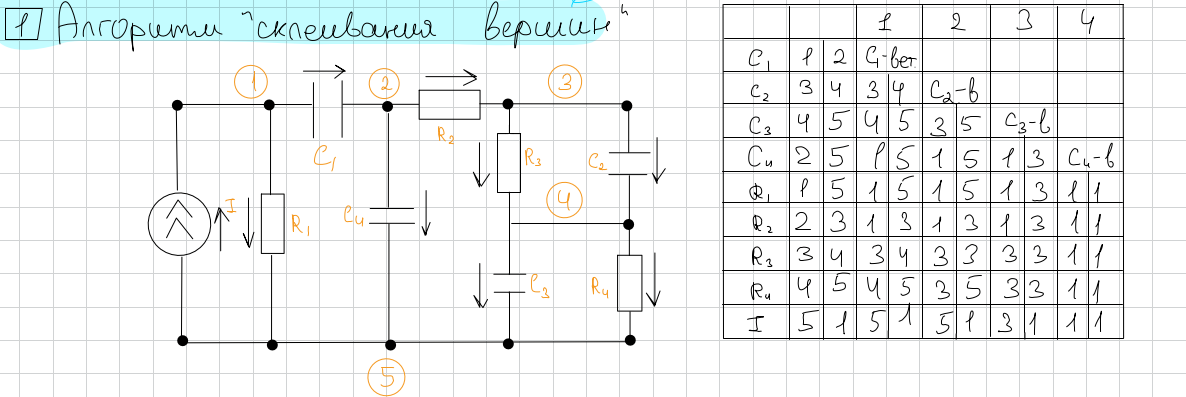
\includegraphics[width=1\linewidth, height=0.2\textheight]{img/25_01}
		\label{fig:25_01}
	\end{figure}
	
	\begin{figure}[H]
		\centering
		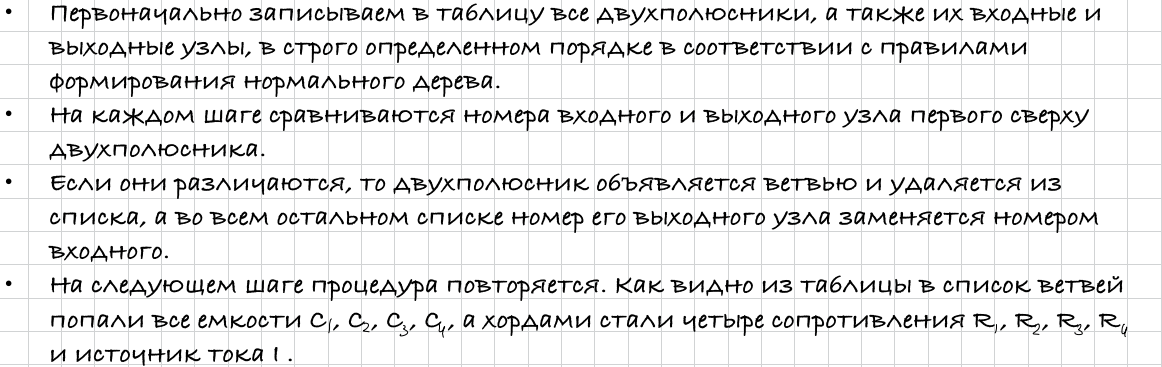
\includegraphics[width=1\linewidth, height=0.2\textheight]{img/25_02}
		\label{fig:25_02}
	\end{figure}
	
	После определения списка ветвей и хорд переходят к этапу 2 и заполняют матрицу 
	контуров и сечений M в соответствии со следующим алгоритмом.
	
	\subsection{Алгоритм <<обрезания вершин>>}
	
	\begin{figure}[H]
		\centering
		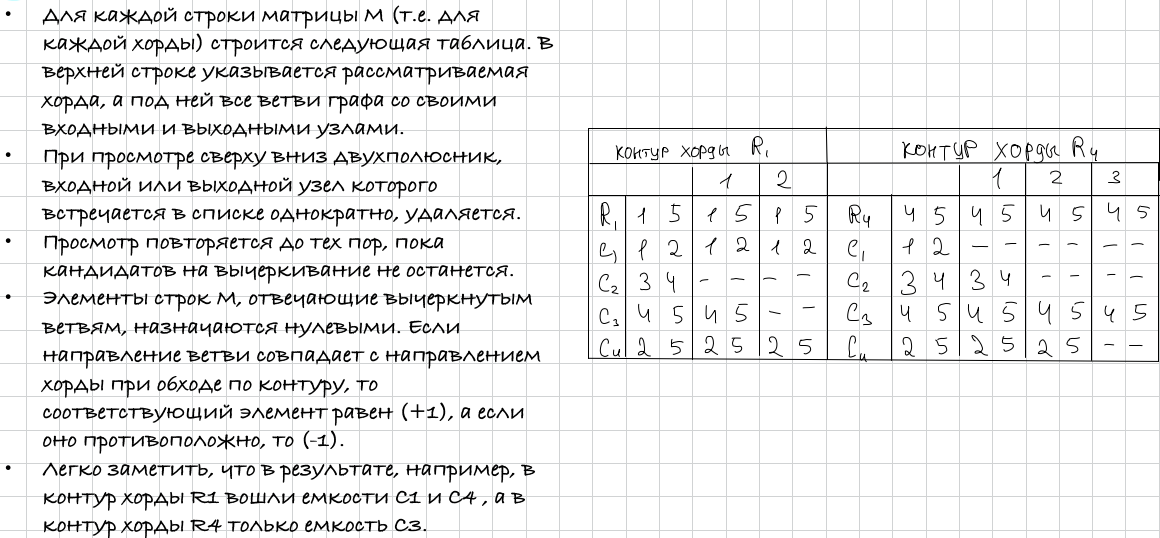
\includegraphics[width=1\linewidth, height=0.2\textheight]{img/25_03}
		\label{fig:25_03}
	\end{figure}
	
	\newpage
	
	% Далее билеты от егорыча
	
	\section{Элементы теории возмущений. Приведение уравнений к безразмерной форме. Возмущения по координате ( \(x \to 0\), \(x \to \infty\)).}
	
	Теория возмущений изучает ситуации, когда существует малый или большой параметр $\varepsilon$ ($\varepsilon \to 0$, $\varepsilon \to \infty$), который возникает в уравнениях естественно или вводится искусственно. 
	
	Все дальнейшие билеты мы будем учиться раскладывать решение всех диффур по этому параметру $\varepsilon$. Зачем? без понятия
	
	\subsection{Приведение уравнения к безразмерной форме}
	
	Операция нужна для того, чтобы "понятие малый или большой стало более определенным"
	
	Пример:
	
	\begin{equation}
		m \frac{d^2u}{dt^2} + ku + k_2u^3 = 0, \; u(0) = u_0, \; \frac{du}{dt}(0) = 0
	\end{equation}
	
	Это модель колебаний тележке на нелинейной пружине. Величины m, u, k и другие имеют вполне определенные физические размерности. Преподавателем предлагается избавиться от размерностей через следующую замену переменных
	
	$$
	u = \frac u {u_0}, \; \tau = \omega_0t, \; \omega_o = \sqrt{\frac k m }
	$$
	Уравнение приобретает вид:
	
	\begin{equation}
		\frac{d^2u}{d\tau^2} + u + \varepsilon u^3 = 0, \; u(0) = 1, \; \frac {du}{dt}(0) = 0, \; \varepsilon = \frac {k_2 u_0^2} {k}
	\end{equation}
	
	\subsection{Возмущение по координате}
	
	Здесь препод резко переобувается в воздухе и заменяет обозначение. $\varepsilon \Rightarrow x$. Говорим о $x$ как о возмущении. Допустим для некоторого $x_0$ решение существует в принципе.
	
	Тогда мы пытаемся найти разложение решения диффуры по степеням $x$. Зачем? Пока загадка
	
	\textbf{Пример 1, $x\to0$:}
	
	\begin{equation}
		x \frac{d^2 u} {dx^2} + \frac {du} {dx} + xu = 0, \; u_0(0) = 1
		\label{eq:perturbation_example_1}
	\end{equation}
	
	Искать будем в виде:
	
	\begin{equation}
		u(x) = \sum_{k=0}^\infty a_k x^{k+\mu}
		\label{eq:series_approximation_example_1}
	\end{equation}
	
	\textit{Уравнение валится с неба, почему именно оно, не объясняется}. $a_k$ и $\mu$ - параметры. Подставляем \eqref{eq:series_approximation_example_1} в \eqref{eq:perturbation_example_1}, получим:
	
	\begin{equation}
		\sum_{k=0}^\infty (\mu + k) (\mu + k - 1) \cdot a_k \cdot x^{\mu + k - 1} + \sum_{k = 0} ^ \infty (\mu + k) \cdot a_k \cdot x^{\mu + k - 1} \sum_{k=0}^\infty a_k \cdot x^{\mu + k + 1} = 0
	\end{equation}
	
	\begin{equation}
		\sum_{k=0}^\infty (\mu + k)^2 \cdot a_k \cdot x^{\mu + k - 1}
		+ \sum_{k = 0}^\infty a_k \cdot x ^ {\mu + k + 1} = 0
	\end{equation}
	
	Первую сумму можно объединить со второй, если вытащить из первой 2 первых члена суммы. Тогда степени x совпадут:
	
	\begin{equation}
		\mu^2 a_0 x^{\mu-1} + (\mu + 1)^2 + \sum_{k=0}^\infty \left [ (\mu + k + 2)^2 a_{k+2} + a_k \right] = 0
	\end{equation}
	
	Наиболее простой способ точно решить это уравнение - взять множитель при степени x и приравнять его к нулю. В данном примере возможны 2 варианта:
	
	\begin{equation}
		\mu = 0, \;
		a_0 = 1, \;
		a_1 = 0, \;
		a_{k+2} = -\frac{a_k}{(k+2)^2}, \;
		u(x) = 1 - \frac {x^2} {2^2} + \frac{x^4}{2^2 4^2} - \frac {x^6}{2^24^26^2} + \dots
	\end{equation}
	
	\begin{equation}
		a_0 = 0, \;
		\mu = -1, \;
		a_1 = 1, \;
		a_{k+2} = - \frac {a_k} {(k+1)^2}, \;
		u(x) = 1 - \frac {x^2} {2^2} + \frac{x^4}{2^2 4^2} - \frac {x^6}{2^24^26^2} + \dots
	\end{equation}
	
	\textbf{Пример 2, $x \to \infty$:}
	
	\begin{equation}
		\frac {du} {dx} + u = \frac 1 x
		\label{eq:perturbation_example_2}
	\end{equation}
	
	Теперь искать разложение по x будем в виде:
	
	\begin{equation}
		u = \sum_{k=1}^\infty a_k x^{-k}
		\label{eq:series_approximation_example_2}
	\end{equation}
	
	Подставляя \eqref{eq:series_approximation_example_2} в \eqref{eq:perturbation_example_2} получаем:
	
	\begin{equation}
		- \sum_{k=1}^\infty k \cdot a_k x^{-k-1} + \sum_{k=2}^\infty a_k x^{-k} + (a_1 - 1) \frac 1 x = 0,
	\end{equation}
	
	\begin{equation}
		a_1 = 1, \; a_{k+1} = ka_k, \; u(x) = \frac 1 x + \frac {1!} {x^2} + \frac {2!}{x^3} + \dots + \frac {(n-1)!}{x^n} + \dots
	\end{equation}
	
	\newpage
	
	\section{Символы порядка и калибровочные функции. Асимптотические разложения, последовательности и ряды}
	
	\subsection{Символы порядка и калибровочные функции}
	
	При сравнении двух функций $f(\varepsilon)$ и $g(\varepsilon)$ используются понятия О-большого и О-малого: $O(\varepsilon)$, $o(\varepsilon)$
	
	\subsubsection{Определения}
	
	$f(\varepsilon) = O(g(\varepsilon))$ при $\varepsilon \to 0$, если $$(\exists A > 0)(\exists \varepsilon_0 > 0)\bigl((\forall \varepsilon > \varepsilon_0)\bigl(|f(\varepsilon)| \leq A \cdot |g(\varepsilon)|\bigr)\bigr)$$ Или $$\lim_{\varepsilon \to 0} \left| \frac{f(\varepsilon)}{g(\varepsilon)} \right| < \infty$$
	
	$f(\varepsilon) = o(g(\varepsilon))$ при $\varepsilon \to 0$, если $$(\exists \delta > 0)(\exists \varepsilon_0 > 0)\bigl((\forall \varepsilon > \varepsilon_0)\bigl(|f(\varepsilon)| \leq \delta \cdot |g(\varepsilon)|\bigr)\bigr)$$ Или $$\lim_{\varepsilon \to 0} \left| \frac{f(\varepsilon)}{g(\varepsilon)} \right| = 0$$
	
	\textit{\textbf{NB}: в кванторах все совпадает посимвольно. Такое же посимвольное совпадение и в методичке. Однако мне кажется что это ошибка. Попробуйте через гугл понять эти 2 понятия}
	
	На практике этого оказывается мало. Обычно ситуация может быть следующая следующая:
	
	\begin{equation}
		\lim_{\varepsilon \to 0} f(\varepsilon) =
		\begin{cases}
			0 \\
			A \neq 0 \\
			\pm \infty
		\end{cases}.
	\end{equation}
	
	Чтобы узнать скорость сходимости, мы сравниваем поведение функции с поведением калибровочных функций. Изначально мы берем их как степени некоего $\varepsilon$:
	
	\[
	\dots, \varepsilon^{-n}, \dots, \varepsilon^{-2}, \varepsilon^{-1}, 1, \varepsilon, \varepsilon^2, \dots, \varepsilon^n, \dots
	\]
	
	Однако не всегда этих функций достаточно, чтобы что-то сказать о скорости сходимости. В общем случае доказывается теорема, что никакого множества калибровочных функций не хватит для того, чтобы описать скорость сходимости в общем случае, поэтому они подбираются под задачу.
	
	Преподаватель демонстрирует несостоятельность степеней $\varepsilon$ на следующем примере: $e^{-\frac 1 \varepsilon}$:
	
	\begin{equation}
		\lim_{\varepsilon \to 0^+} \frac{\varepsilon^n}{e^{-\frac{1}{\varepsilon}}} = \lim_{x \to \infty} \frac{x^n}{e^x} = 0
	\end{equation}
	
	Если попытаться расширить список калибровочных функций например при помощи $\ln\left(\frac 1 \varepsilon \right)$, то найдется другой пример:
	
	\begin{equation}
		\lim_{\varepsilon \to 0^+} \frac{\ln\left(\frac{1}{\varepsilon}\right)}{\varepsilon^{-\alpha}} = \lim_{x \to \infty} \frac{\ln(x)}{x^\alpha} = \lim_{x \to \infty} \frac{1}{x \cdot \alpha \cdot x^{\alpha-1}} = \frac{1}{\alpha} \lim_{x \to \infty} \frac{1}{x^\alpha} = 0, \quad \forall \alpha > 0
	\end{equation}
	
	Снова не получается. Может прийти в голову желание еще раз расширить набор калибровочных функций, добавив $\ln\left(\ln\left(\frac 1 \varepsilon\right)\right)$, однако этот процесс никогда не закончится. \textit{Универсального списка калибровочных функций для всех всегда навсегда не существует}
	
	\textbf{В конечном итоге список калибровочных функций подбирается под задачу индивидуально}
	
	\subsection{Асимптотические разложения, последовательности и ряды}
	
	\textbf{Суть:} При помощи только что рассмотренных разложений можно с какой-то неплохой точностью приближать интеграллы
	
	\subsubsection{Демонстрация}
	
	Начнем с примера
	
	\begin{equation}
		1 > F(x) = \int_0^\infty \frac{e^{-t}}{1 + xt} \, dt \implies \sum_{k=0}^\infty (-1)^k k! x^k
	\end{equation}
	
	Как видно здесь $x$ - параметр возмущения. В целом ряд расходится, однако ряд знакопеременный. Если вы помните еще что-то из вышмата, то в таком ряду для любой частной суммы из первых $n$ элементов погрешность не превышает первый отброшенный (n+1) элемент по модулю
	
	Тогда если $x = 0.1$, то для $n=10$ погрешность составит $10!\cdot0.1^{10} \approx 0.000363$
	
	\subsubsection{Обобщение}
	
	Если функцию $f(\varepsilon)$ можно представить в виде:
	
	\begin{equation}
		f(\varepsilon) = \sum_{k=0}^N a_k \varepsilon^k + o\bigl(\varepsilon^N\bigr) \quad \text{при } \varepsilon \to 0,
		\label{eq:asymptotic_series_Puancare}
	\end{equation}
	
	то \eqref{eq:asymptotic_series_Puancare} называют \textbf{асимптотическим рядом типа Пуанкаре}
	
	\vspace{1em}
	
	Вместо $\varepsilon^k$ может стоять все, что удовлетворяет свойству $\delta_k(\varepsilon) = o\left[\delta_{k-1}(\varepsilon)\right]$, при $\varepsilon \to 0$. В итоге \eqref{eq:asymptotic_series_Puancare} перепишется в виде:
	
	\begin{equation}
		f(\varepsilon) = \sum_{k=0}^{N} a_k \delta_k(\varepsilon) + o(\delta_N(\varepsilon)), \quad \varepsilon \to 0
	\end{equation}
	
	В роли $\delta_k(\varepsilon)$ могут быть $\varepsilon^k$, $\varepsilon^{\frac k {10}}$, $(\ln(\varepsilon)^{-k}$ и т.п.
	
	\newpage
	
	\section{Возмущения по параметру: алгебраические уравнения (регулярный случай с различными и кратными корнями, сингулярный случай), трансцендентные уравнения, дифференциальные уравнения (регулярный случай, методика растянутых параметров Линдштедта-Пуанкаре, сингулярный случай, сращивание асимптотических разложений)}
	
	\subsection{СКИИИИИПААААААЕЕЕЕЕЕМ}
	
	\newpage
	
	\section{Упрощение математических моделей, описываемых жесткими дифференциальными уравнениями. Принцип квазистационарности производных (ПКП)}
	
	\subsection{Упрощение математических моделей, описываемых жесткими дифференциальными уравнениями}
	
	Рассмотрим некий небольшой параметр $\varepsilon$ и систему диффур:
	\vspace{-0.7em}
	\begin{align}
		&\varepsilon \frac{dx_1}{dt} = -\left(1 + \varepsilon^2\right)x_1 - \left(1 - \varepsilon^2\right)x_2 \\
		&\frac{dx_2}{dt} = x_1
	\end{align}
	
	Перепишем в матричной форме:
	
	\begin{equation}
		\frac{d\mathbf{x}}{dt} = \mathbf{A} \cdot \mathbf{x}, \quad
		\mathbf{A} = 
		\begin{pmatrix}
			-\frac{1 + \varepsilon^2}{\varepsilon} & -\frac{1 - \varepsilon^2}{\varepsilon} \\
			1 & 0
		\end{pmatrix}.
	\end{equation}
	
	Вычисляем собств. значения: $\lambda_1 = -1 - \varepsilon$, $\lambda_2 = - \frac 1 \varepsilon + 1$. Из-за малости $\varepsilon$ система является жесткой
	
	В инженерной практике нередко решают пренебречь производной $\varepsilon \frac {x_1}{dt}$, таким образом превращая уравнение в алгебраическое
	\vspace{-0.85em}
	\begin{align}
		&-(1+\varepsilon^2)x_1 - (1-\varepsilon^2)x_2 \approx 0, \\
		&\frac{dx_2}{dt} = x_1 \approx \frac{-(1-\varepsilon^2)}{(1+\varepsilon^2)}x_2 \approx (-1 + 2\varepsilon^2 + \dots)x_2.
	\end{align}
	
	Заметим, что коэффициент $(-1 + 2\varepsilon^2 + \dots)$, дающий нам в характерристическом уравнении степени экоспоненты, с точностью до $\varepsilon$ совпадает с $\lambda_1 = - 1 - \varepsilon$
	
	\vspace{1em}
	
	Хорошо себя показывает этот метод и в следующем примере:
	
	\vspace{-0.85em}
	
	\begin{align}
		10^{-3} \cdot \frac{dx_1}{dt} &= -x_1 + 0.999x_2, \\
		\frac{dx_2}{dt} &= x_1 - 2x_2 \tag{10}.
	\end{align}
	
	Если разделить первое уравнение (10) на $10^{-3}$, то матрица получившейся системы обладает следующими собственными значениями: $\lambda_1 = -1$, $\lambda_2 = -1001$. В соответствии с «инженерным подходом» пренебрегаем слагаемым $10^{-3} \cdot \frac{dx_1}{dt}$ в первом уравнении и получаем
	\begin{align*}
		& -x_1 + 0.999x_2 \approx 0, \\
		& \frac{dx_2}{dt} = x_1 - 2x_2 \approx -1.001 \cdot x_2.
	\end{align*}
	И вновь, как и в предыдущем примере, значение $-1.001$ оказывается весьма близким к $\lambda_1 = -1$.
	
	Однако, применение такого подхода на практике сталкивается со следующими трудностями:
	
	\begin{itemize}
		\item Трудно оценить погрешность такого пренебрежения малым параметром;
		\item Трудно уменьшить эту погрешность, если она недостаточно мала;
		\item Количество уравнений с малым параметром при производной может не совпадать с количеством быстроубывающих в пограничном слое составляющих решения.
	\end{itemize}
	
	\newpage
	
	Рассмотрим последний пункт на следующем примере
	
	\begin{equation}
		\frac{d\mathbf{x}}{dt} = \mathbf{A} \cdot \mathbf{x}, \quad 
		\mathbf{A} = \begin{pmatrix}
			-501 & 500 \\
			500 & -501
		\end{pmatrix}, \quad t \in [0, 3]
		\label{eq:leaving_derivatives_bad_example}
	\end{equation}
	
	Если разделить оба уравнения на 1000, то получается два уравнения с малым параметром при производной и складывается впечатление, что матрица обладает двумя большими по модулю собственными значениями, соответствующие две экспоненты быстро исчезают в пределах пограничного слоя, и решение почти на всем промежутке $t \in [0, 3]$ оказывается равным нулю. Однако собственные значения $\mathbf{A}$ равны: $\lambda_1 = -1$, $\lambda_2 = -1001$. Таким образом, пренебрегая малым параметром в обоих уравнениях, мы ошибочно удаляем из решения вне пограничного слоя экспоненту с показателем $\lambda_1 = -1$. даже если это учесть и пренебрегать малым параметром лишь в одном уравнении, то это приводит к следующему результату:
	
	\begin{equation}
		x_1 \approx \frac{500}{501} x_2, \quad
		\frac{dx_2}{dt} \approx -\left( 501 - \frac{500^2}{501} \right) x_2 = -\frac{1001}{501} x_2 \approx -2 x_2.
	\end{equation}
	
	Согласно этому $\lambda_1 = -2$, что в 2 раза отличается от правды
	
	\subsection{Принцип квазистационарности производных (ПКП)}
	
	Суть в том, чтобы отбрасывать не первую производную, а следующие. На основе уже рассмотренной системы \eqref{eq:leaving_derivatives_bad_example}, продифференцируем первое уравнение по $dt$ и пренебрежем уже второй производной $\left(\frac{d^2x_1}{dt^2}\approx 0\right)$
	
	\begin{align}
		0 &\approx \frac{d^2 x_1}{dt^2} = -501 \frac{dx_1}{dt} + 500 \frac{dx_2}{dt} = -501(-501x_1 + 500x_2) + 500(500x_1 - 501x_2), \\
		x_1 &\approx \frac{1000 \cdot 501}{501^2 + 500^2} x_2, \quad \frac{dx_2}{dt} \approx -\left( 501 - \frac{500 \cdot 501}{501^2 + 500^2} \right) x_2 \approx -1.001 x_2.
	\end{align}
	
	То есть $\lambda_1 = -1.001$ - погршеность в 3 знаке - неплохо
	
	\subsubsection{Более формальная демонстрация}
	
	\begin{align}
		\varepsilon \frac{d\mathbf{x}_1}{dt} &= \mathbf{f}_1(\mathbf{x}_1, \mathbf{x}_2), \\
		\frac{d\mathbf{x}_2}{dt} &= \mathbf{f}_2(\mathbf{x}_1, \mathbf{x}_2),
	\end{align}
	
	Из любопытства сначала, как и раньше, отбросим первую производную с малым коэффициентом при ней
	
	\begin{equation}
		\mathbf{f}_1(\mathbf{x}_1, \mathbf{x}_2) \approx 0.
	\end{equation}
	
	Теперь продифференцируем первое уравнение и пренебрежем второй производной:
	
	\begin{equation}
		0 \approx \varepsilon \frac{d^2 \mathbf{x}_1}{dt^2} = \frac{\partial \mathbf{f}_1}{\partial \mathbf{x}_1} \frac{d\mathbf{x}_1}{dt} + \frac{\partial \mathbf{f}_1}{\partial \mathbf{x}_2} \frac{d\mathbf{x}_2}{dt} = \frac{\partial \mathbf{f}_1}{\partial \mathbf{x}_1} \frac{\mathbf{f}_1(\mathbf{x}_1, \mathbf{x}_2)}{\varepsilon} + \frac{\partial \mathbf{f}_1}{\partial \mathbf{x}_2} \mathbf{f}_2(\mathbf{x}_1, \mathbf{x}_2).
	\end{equation}
	
	Здесь алгебраическое уравнение вне пограничного слоя выглядит следующим образом
	
	\begin{equation}
		\mathbf{f}_1(\mathbf{x}_1, \mathbf{x}_2) + \varepsilon \left( \frac{\partial \mathbf{f}_1}{\partial \mathbf{x}_1} \right)^{-1} \frac{\partial \mathbf{f}_1}{\partial \mathbf{x}_2} \mathbf{f}_2(\mathbf{x}_1, \mathbf{x}_2) \approx 0.
	\end{equation}
	
	Таким образом относительно первого разложения мы получили поправку порядка $\varepsilon$
	
	\newpage
	
	\subsubsection{Доказательство для линейных систем}
	
	Пусть для простоты только одно собственное значение сильно меньше остальных. Продифференцируем $S$ раз и пренебрежем $S$-й производной в уравнении с номером $j$:
	
	\[
	\frac{d^2 \mathbf{x}}{dt^2} = \mathbf{A} \frac{d\mathbf{x}}{dt}, \quad \frac{d^S \mathbf{x}}{dt^S} = \mathbf{A}^S \mathbf{x},
	\]
	
	\begin{equation}
		0 \approx \frac{d^S x_j}{dt^S} = -e_j^T \mathbf{A}^S \mathbf{x} = \sum_{k=1}^{m} \left( \mathbf{e}_j^T \mathbf{u}_k \right) \mathbf{v}_k^T \lambda_k^S \mathbf{x} = \sum_{k=1}^{m} \left( \mathbf{e}_j^T \mathbf{u}_k \right) \mathbf{v}_k^T \lambda_k^S \mathbf{x} =
	\end{equation}
	
	\[
	= \lambda_j^S \left( \left( \mathbf{e}_j^T \mathbf{u}_1 \right) \mathbf{v}_1^T \mathbf{x} + \sum_{k=2}^{m} \left( \mathbf{e}_j^T \mathbf{u}_k \right) \frac{\lambda_k^S}{\lambda_j^S} \mathbf{v}_k^T \mathbf{x} \right).
	\]
	
	Так как $\left| \frac{\lambda_k^S}{\lambda_j^S} \right| \ll 1$, то с ростом $S$ сумма в правой части быстро убывает, и все выражение принимает вид:
	
	\begin{equation}
		\lambda_j^S \left( \mathbf{e}_j^T \mathbf{u}_1 \right) \mathbf{v}_1^T \mathbf{x} \approx 0 \Rightarrow \mathbf{v}_1^T \mathbf{x} \approx 0,
	\end{equation}
	
	Погрешность легко оценивается сравнением коэффициентов алгебраических связей для $S$ и $S+1$, а повышение точности достигается увеличением $S$
	
	\newpage
	
	\section{Понятие антиинтуитивных систем, их признаки и типичные ошибки при принятии управленческих решений}
	
	\subsection{Проблемы интуиции}
	\vspace{-1em}
	\begin{figure}[H]
		\centering
		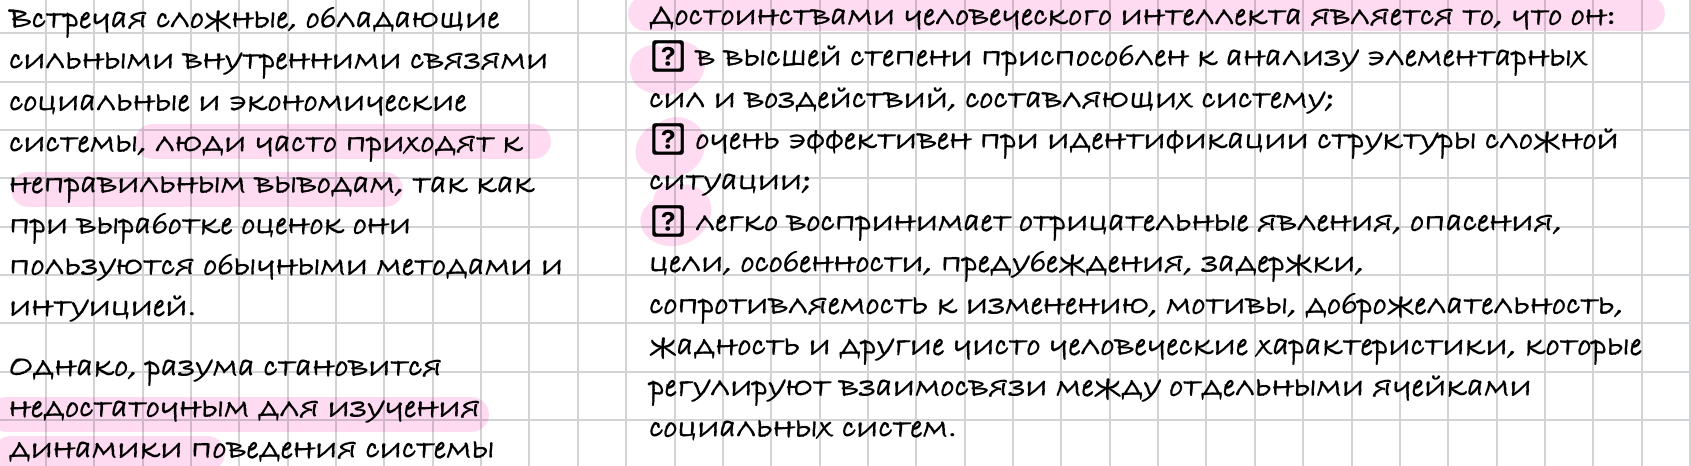
\includegraphics[width=1\linewidth, height=0.2\textheight]{img/30_01}
		\label{fig:30_01}
	\end{figure}
	\vspace{-1em}
	\subsection{Ловушки антиинтуитивных систем}
	\vspace{-1em}
	\begin{figure}[H]
		\centering
		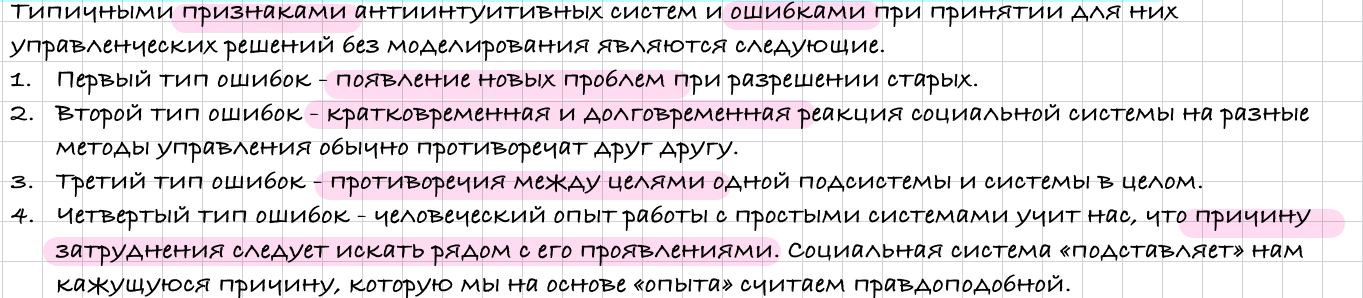
\includegraphics[width=1\linewidth, height=0.2\textheight]{img/30_02}
		\label{fig:30_02}
	\end{figure}
	\vspace{-1em}
	\subsection{Пример модели Вольмерра <<хищник-жертва>>}
	
	\[
	\left\{
	\begin{aligned}
		\frac{dr}{dt} &= 2r - \alpha rf \\
		\frac{df}{dt} &= \alpha rf - f
	\end{aligned}
	\right.
	\qquad
	\begin{aligned}
		&r \text{ — кролики} \\
		&f \text{ — лисы} \\
		&\alpha  \text{ — вероятность смерти} \\
		&\text{система — их совместное существование}
	\end{aligned}
	\]
	\vspace{-1em}
	\begin{figure}[H]
		\centering
		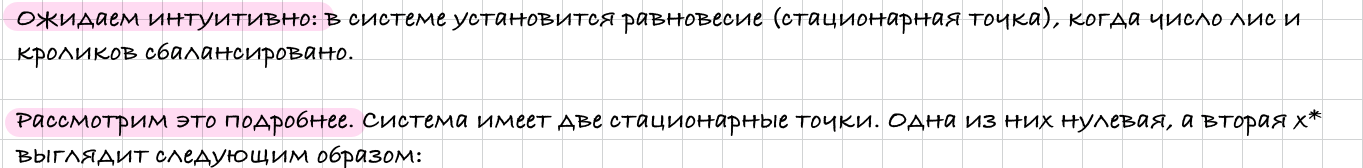
\includegraphics[width=1\linewidth, height=0.1\textheight]{img/30_03}
		\label{fig:30_03}
	\end{figure}
	\vspace{-1em}
	\[
	\vec{x} = 
	\begin{pmatrix}
		r \\
		f
	\end{pmatrix}, \qquad
	x^* = 
	\begin{pmatrix}
		\frac{1}{\alpha} \\
		\frac{2}{\alpha}
	\end{pmatrix}, \qquad
	J = 
	\begin{pmatrix}
		2 - \alpha f & -\alpha r \\
		\alpha f & -1 + \alpha r
	\end{pmatrix}, \qquad
	J(x^*) = 
	\begin{pmatrix}
		0 & -1 \\
		2 & 0
	\end{pmatrix}
	\]
	
	\[
	\lambda_{1,2} = \pm i\sqrt{2}
	\]
	\newpage
	\begin{figure}[H]
		\centering
		
\includegraphics[width=1\linewidth, height=0.2\textheight]{img/30_04}
		\label{fig:30_04}
	\end{figure}
	\vspace{-2.5em}
	\subsection{Проблема социально-экономических моделей}
	\vspace{-1em}
	\begin{figure}[H]
		\centering
		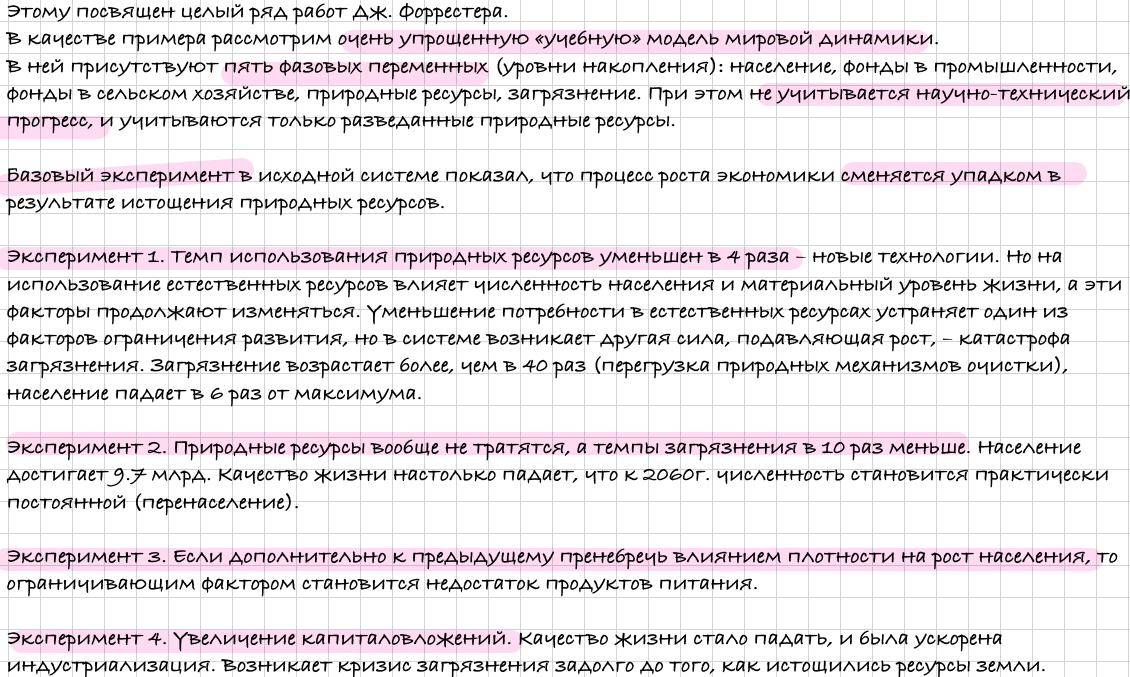
\includegraphics[width=1\linewidth, height=0.35\textheight]{img/30_05}
		\label{fig:30_05}
	\end{figure}
	\vspace{-2em}
	\begin{figure}[H]
		\centering
		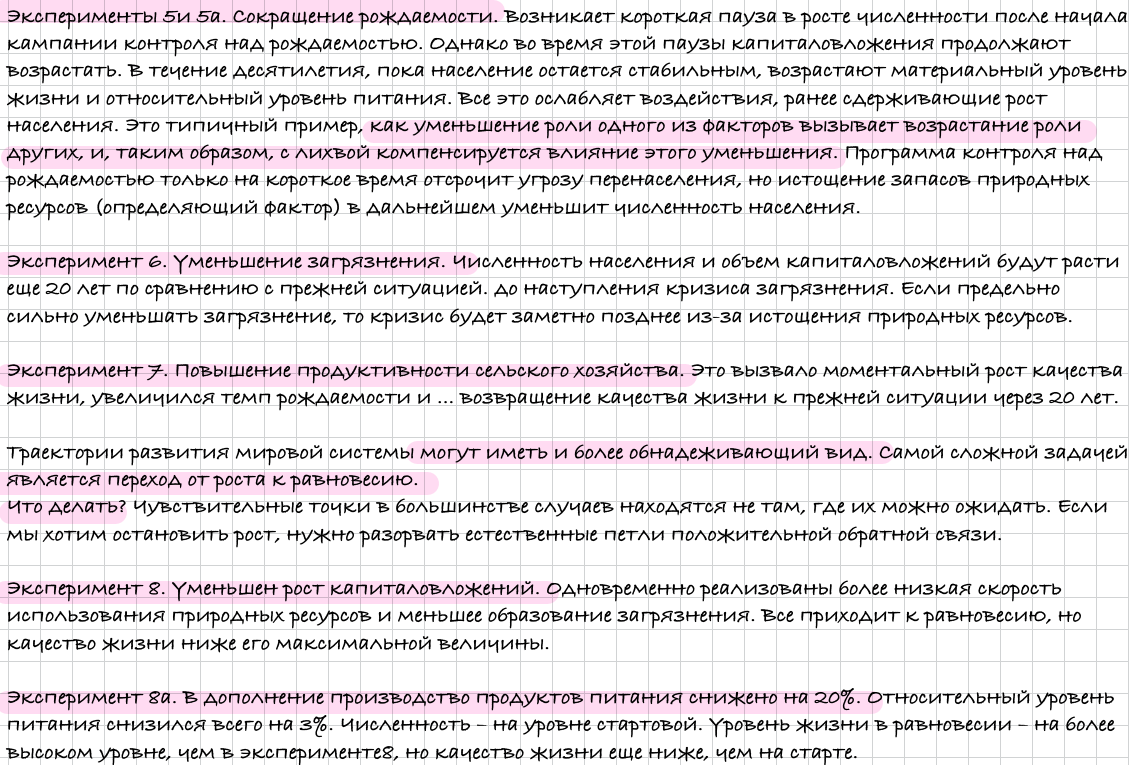
\includegraphics[width=1\linewidth, height=0.35\textheight]{img/30_06}
		\label{fig:30_06}
	\end{figure}
	\newpage
	\subsection{Итоговая модель}
	\vspace{-1em}
	\begin{figure}[H]
		\centering
		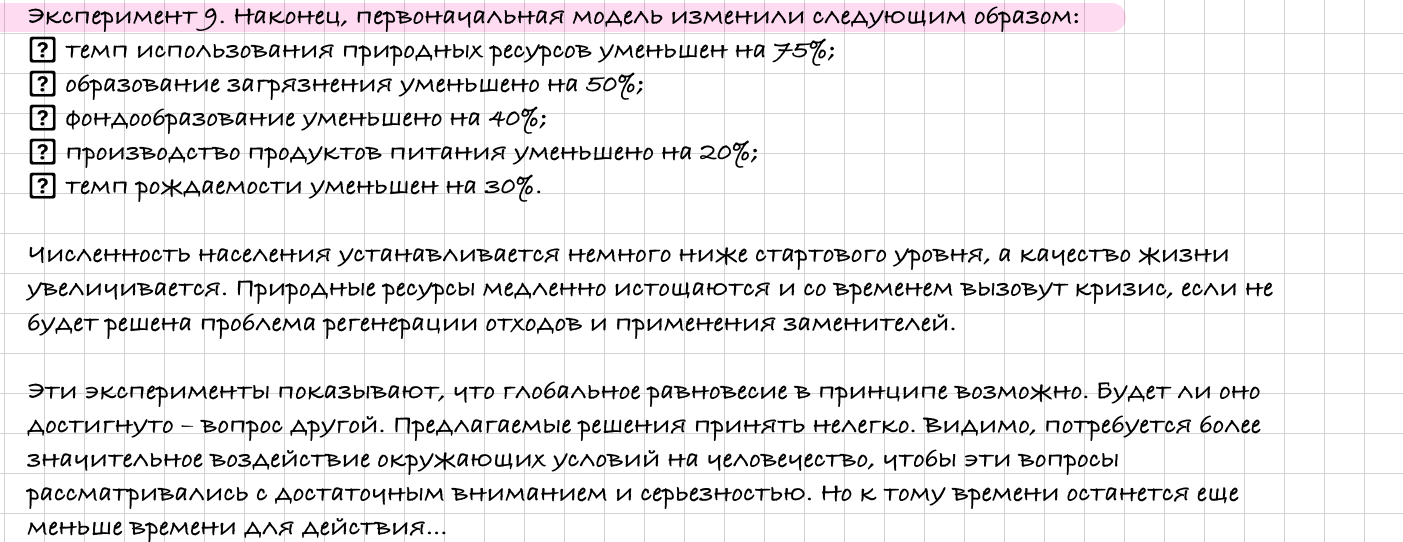
\includegraphics[width=1\linewidth, height=0.2\textheight]{img/30_07}
		\label{fig:30_07}
	\end{figure}
	
\end{document}
